\chapter{SYSTEM INTERFACE AND PHYSICAL DESIGN}
\label{chap:system_interface_physical_design}

This chapter shows what each user sees and how the data is stored. Section~\ref{sec:system_user_interfaces} follows an exam from start to finish: the student's desktop client, exam set-up, live invigilation, evaluation, administration and the student portal. Section~\ref{sec:physical_tables} gives one table for each entity of the ERD (Figure~\ref{fig:erd_diagram}) with its fields, data types and keys.

\section{System User Interfaces}
\label{sec:system_user_interfaces}
SmartExam has two front ends: a WPF desktop client (.NET~9) in which students sit the exam, and a React web panel with one route group per role (\texttt{/admin}, \texttt{/teacher}, \texttt{/invigilator}, \texttt{/student}). Both follow common usability heuristics: the system status is always visible (connection, last save, tile status), final actions such as submit and force-submit ask for confirmation, and controls look the same across roles \cite{nielsen_heuristics}. The web figures are captured from the running panel by a Playwright script (\texttt{Admin\_Web\_Panel/tests/docs}) against the in-memory backend with the seeded demo data; a scripted client plays the desktop app and uploads the screen captures. The desktop figures are rendered off-screen from the client's own XAML (Extensible Application Markup Language) views with values from the same run, because the lockdown window cannot be captured safely on a development PC. The student, invigilation and evaluation figures show one exam, the Mid-Term Lab Exam (Demo), in Enforce mode with a required system check and webcam.

% Section 6.1 is mostly screenshots: let a tall figure share a page with text
% (book defaults are restored before Section 6.2).
\renewcommand{\topfraction}{0.9}\renewcommand{\bottomfraction}{0.9}
\renewcommand{\textfraction}{0.07}\renewcommand{\floatpagefraction}{0.8}
\subsection{Student Desktop Client}
The student signs in with email or roll number (Figure~\ref{fig:ui_student_login}). The client reads the BIOS, system-disk and baseboard serials; the server hashes them with SHA-256 into the hardware ID (HWID) and keeps only the hash in \texttt{DeviceBindings}, so a login from another PC is refused (FR1). The window has one field for the email or roll number (here \texttt{BSCS-21-001}) and one for the password. The note above \emph{Sign In} warns that the device will be bound to the account, and the box at the bottom shows the connection state (\emph{Connected to server}), so the student knows before signing in that the server can be reached.

\begin{figure}[tbp]
\centering
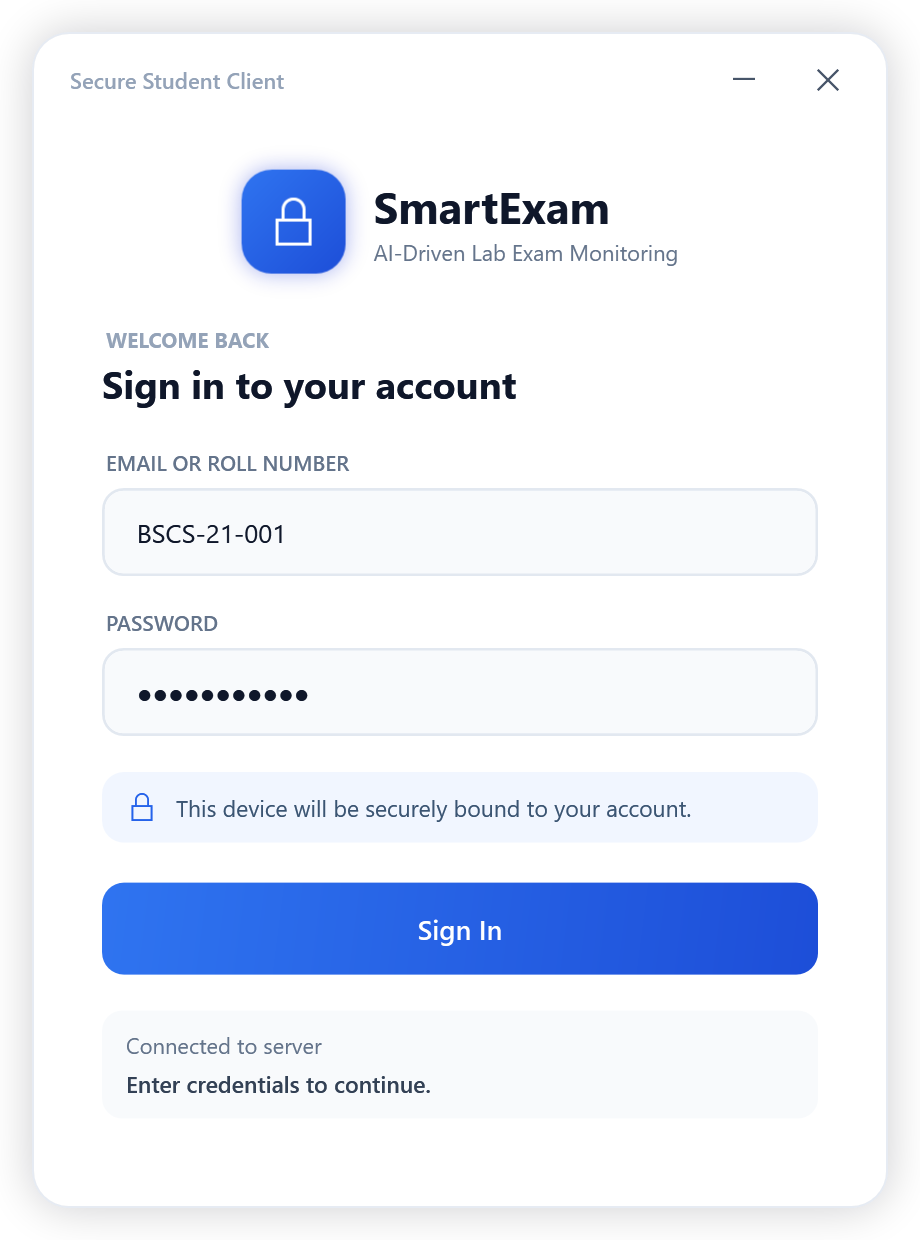
\includegraphics[width=\linewidth,height=0.9\textheight,keepaspectratio]{Figures/ui_student_login.png}
\caption{Desktop Client Login}
\label{fig:ui_student_login}
\end{figure}
\SoftBarrierN

The exam dashboard shows the student's current assigned exam with its instructions and permitted applications (Figure~\ref{fig:ui_student_diagnostics}); a side panel, not shown, gives the remaining time, lab, seat, attendance check-in and invigilator messages. An ineligible student still sees the exam, with \emph{Start Exam} disabled and the reason shown (FR3). In the figure, the blue header gives the exam title, its status (Active) and the teacher (Dr. Ahmed), and the permitted applications are \texttt{code.exe} and \texttt{codeblocks.exe}. In the \emph{System Check} list a green tick is a passed check, a dash is a skipped check and a red cross is a failed check with a \emph{Retry} button beside it. The dashboard runs the readiness checks (FR2): network, clock skew, screen capture, webcam, microphone, secure mode (monitors, remote session, virtual machine, keyboard hook) and disk space. This exam needs the webcam but not the microphone, so the microphone is skipped. Secure mode fails because a second monitor is attached, and since the exam requires the check (\texttt{RequireReadiness}), \emph{Start Exam} stays disabled until a passing check less than 30 minutes old exists.

\begin{figure}[tbp]
\centering
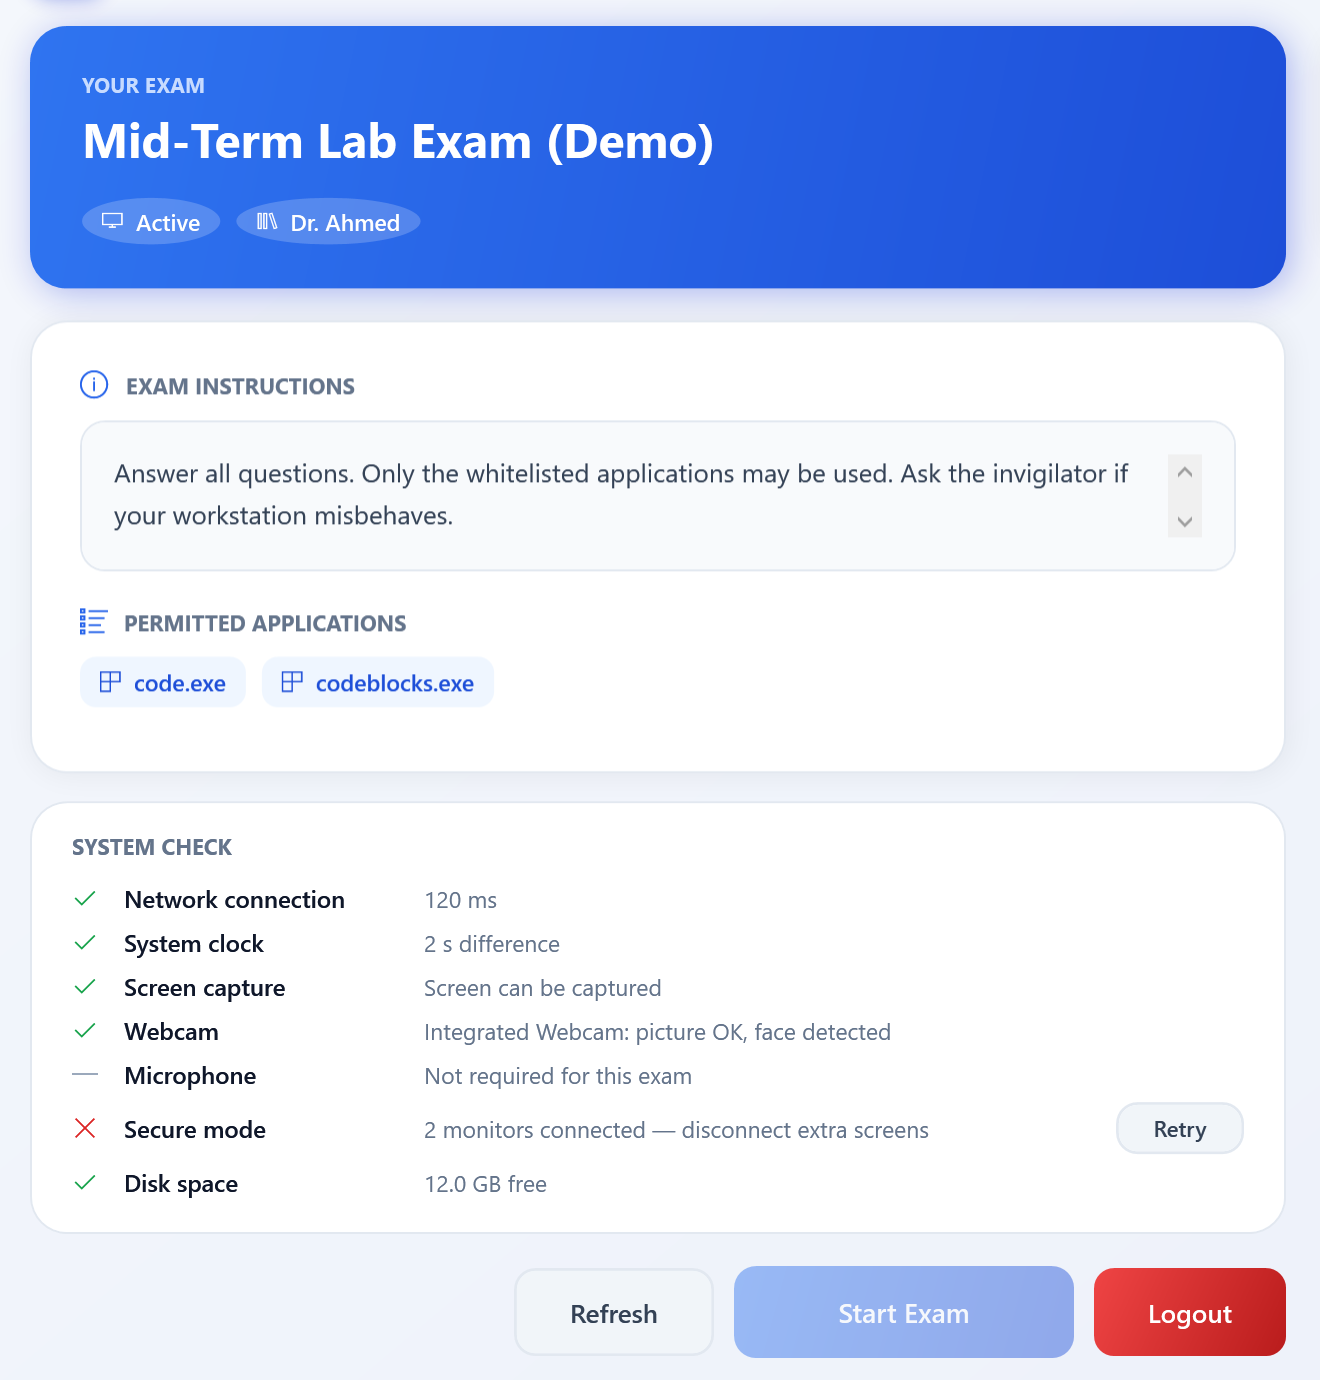
\includegraphics[width=\linewidth,height=472pt,keepaspectratio]{Figures/ui_student_diagnostics.png}
\caption{Exam Dashboard with Readiness Checks}
\label{fig:ui_student_diagnostics}
\end{figure}
\SoftBarrierN

The exam window (Figures~\ref{fig:ui_student_workspace} and~\ref{fig:ui_student_workspace_b}) opens maximised, borderless and topmost (FR4). A low-level keyboard hook blocks the Windows and menu keys, PrintScreen, Alt+Tab, Alt+F4, Alt+Esc, Ctrl+Esc and Ctrl+Shift+Esc, while guard services watch processes, the clipboard and newly mounted USB storage devices. The student picks a question from the list on the left and types the answer; coding answers go into a monospace text box. Every edit is written within about a second to an AES-256-GCM encrypted backup on disk and saved to the server 10~s after the first unsaved edit; saves made offline are queued and replayed (FR6). The footer shows the last save time.

The window is printed in two parts. Part~(a) is the left side panel: the exam title with the number of answered questions (2 of 3), the question list (1 Coding, 2 Theory, 3 Multiple Choice) with a green dot for each answered question, and the footer \emph{Saved 3:35:32 PM}; the empty middle of the panel is cut out. Part~(b) is the question area: the countdown timer (01:27:18) in the header, the type and marks of Question~1 (Coding, 20 marks), the C++ answer in the \emph{Your Code} box, and the \emph{Previous}, \emph{Next} and \emph{Submit Exam} buttons. So the student can always see how much is answered, how much time is left and when the work was last saved.

\begin{figure}[tbp]
\centering
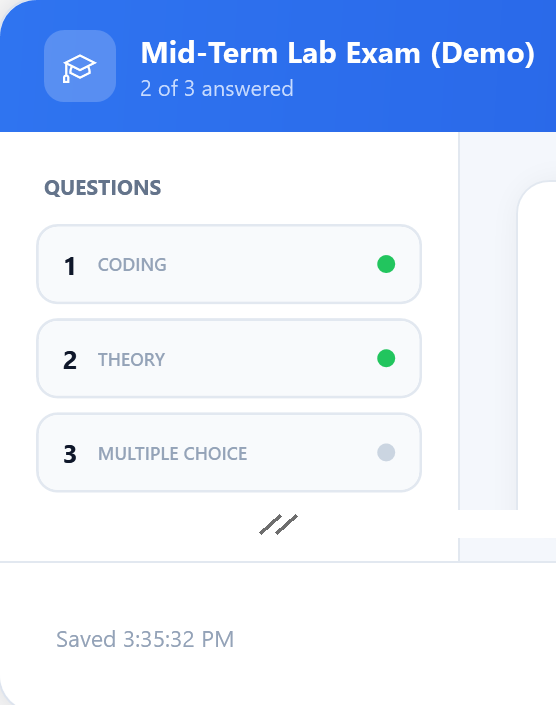
\includegraphics[width=0.5\linewidth]{Figures/ui_student_workspace_p1.png}
\caption{Desktop Exam Window (a): Question List and Save Status (Empty Middle Omitted)}
\label{fig:ui_student_workspace}
\end{figure}
\SoftBarrierN

\begin{figure}[tbp]
\centering
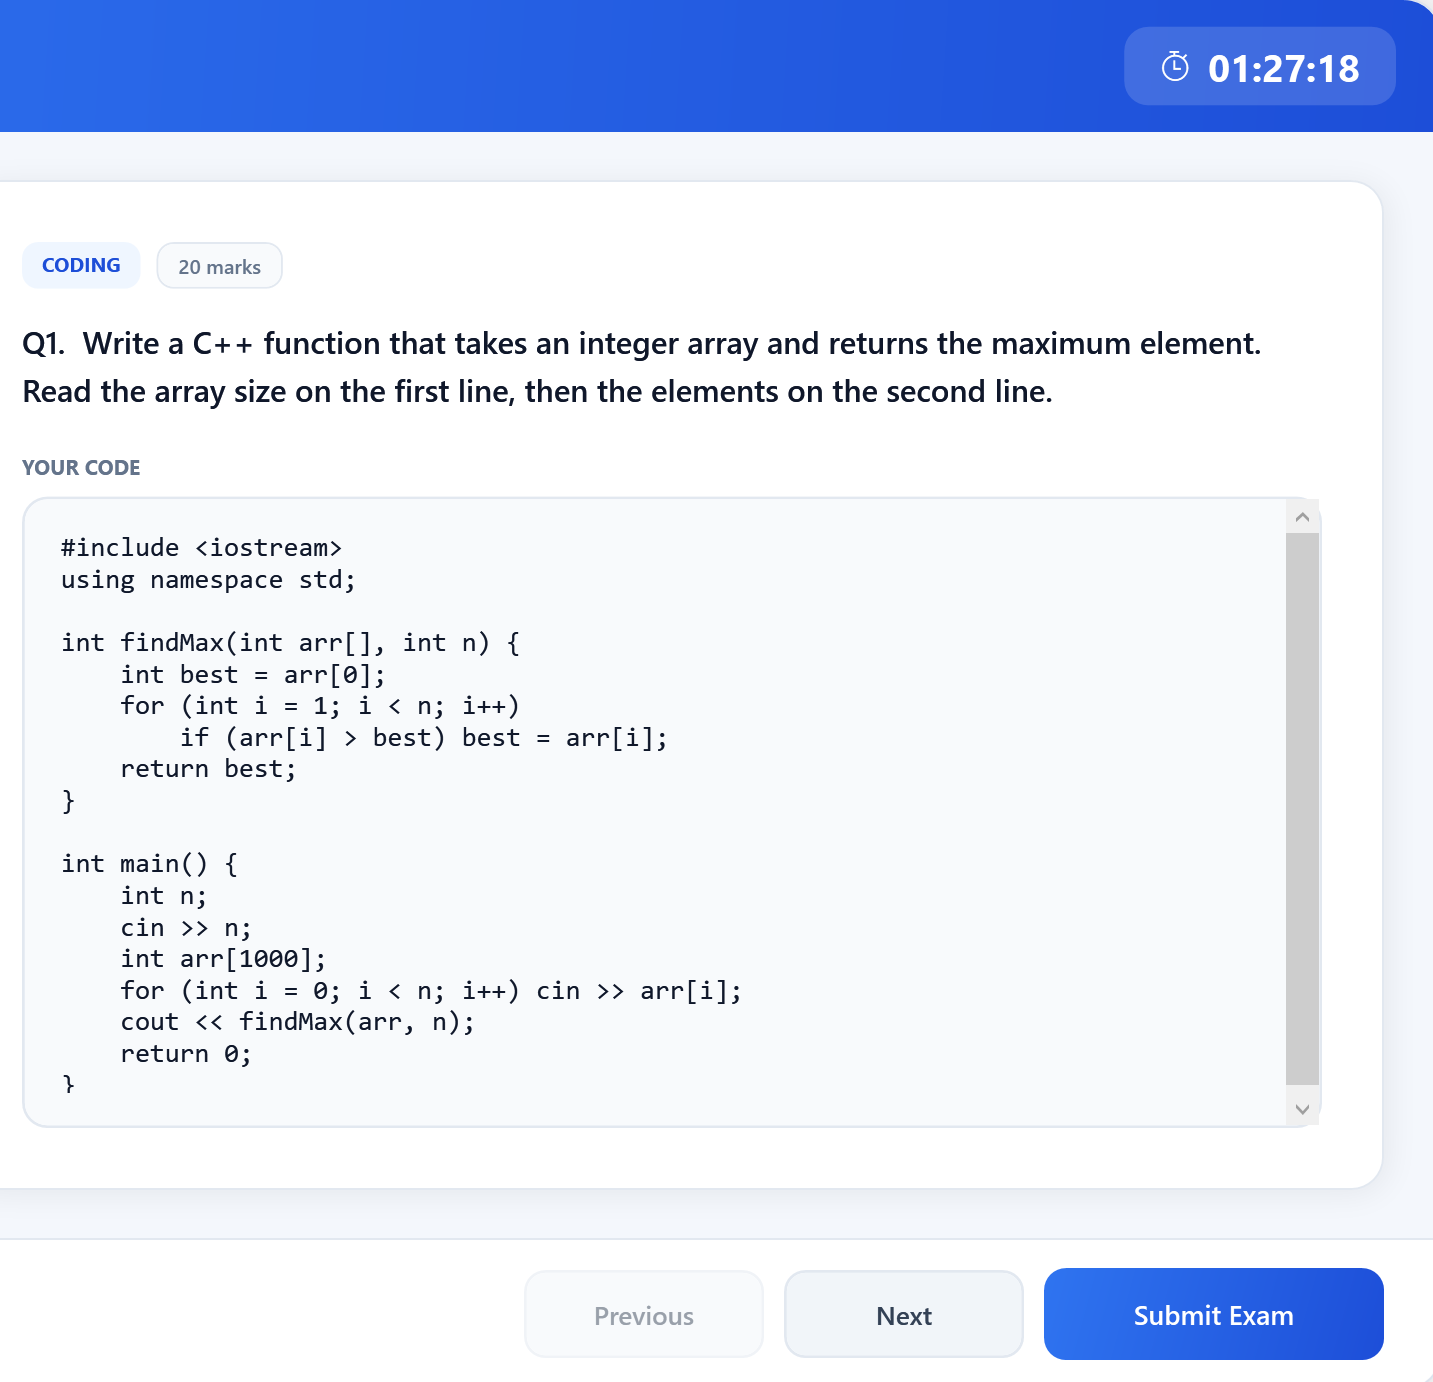
\includegraphics[width=\linewidth]{Figures/ui_student_workspace_p2.png}
\caption{Desktop Exam Window (b): Coding Question, Timer and Answer Box}
\label{fig:ui_student_workspace_b}
\end{figure}
\SoftBarrierN

A warning sent by an invigilator reaches the client in the reply to its next heartbeat (every 10~s) and appears as a banner between the window header and the question (Figure~\ref{fig:ui_student_warning}, the warning sent in Figure~\ref{fig:ui_live_timeline}). The banner shows the title \emph{Proctor Warning} with the time it was sent (15:35), the invigilator's message and an \emph{Acknowledge} button; the empty middle of the wide banner is cut out. The banner stays until the student acknowledges it, further warnings wait in a queue and are shown one by one, and the student's \emph{Acknowledge} is written to the audit log (FR10).

\begin{figure}[tbp]
\centering
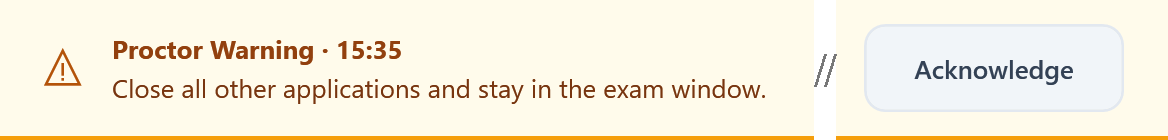
\includegraphics[width=\linewidth]{Figures/ui_student_warning_banner.png}
\caption{Invigilator Warning Banner in the Exam Window (Empty Middle Omitted)}
\label{fig:ui_student_warning}
\end{figure}
\SoftBarrierN

\subsection{Exam Setup}
The teacher dashboard (Figure~\ref{fig:ui_teacher_dashboard}) counts the teacher's exams, the running ones and the ended exams waiting for grade review. It lists scheduled exams, including the seeded practice exam, which stays open for a week, with \emph{Manage}, \emph{Edit} and \emph{Delete}, and links each ended exam to \emph{Review Grades}. In the figure, Dr. Ahmed has six exams, one running now and three waiting for review. The left list holds the two scheduled exams, the practice exam (tagged \emph{Practice}) and the End-Term Lab Exam (tagged \emph{Ready}), and the right panel lists the three ended Data Structures exams. The page tells the teacher at a glance what is coming next and what still needs grading.

\begin{figure}[tbp]
\centering
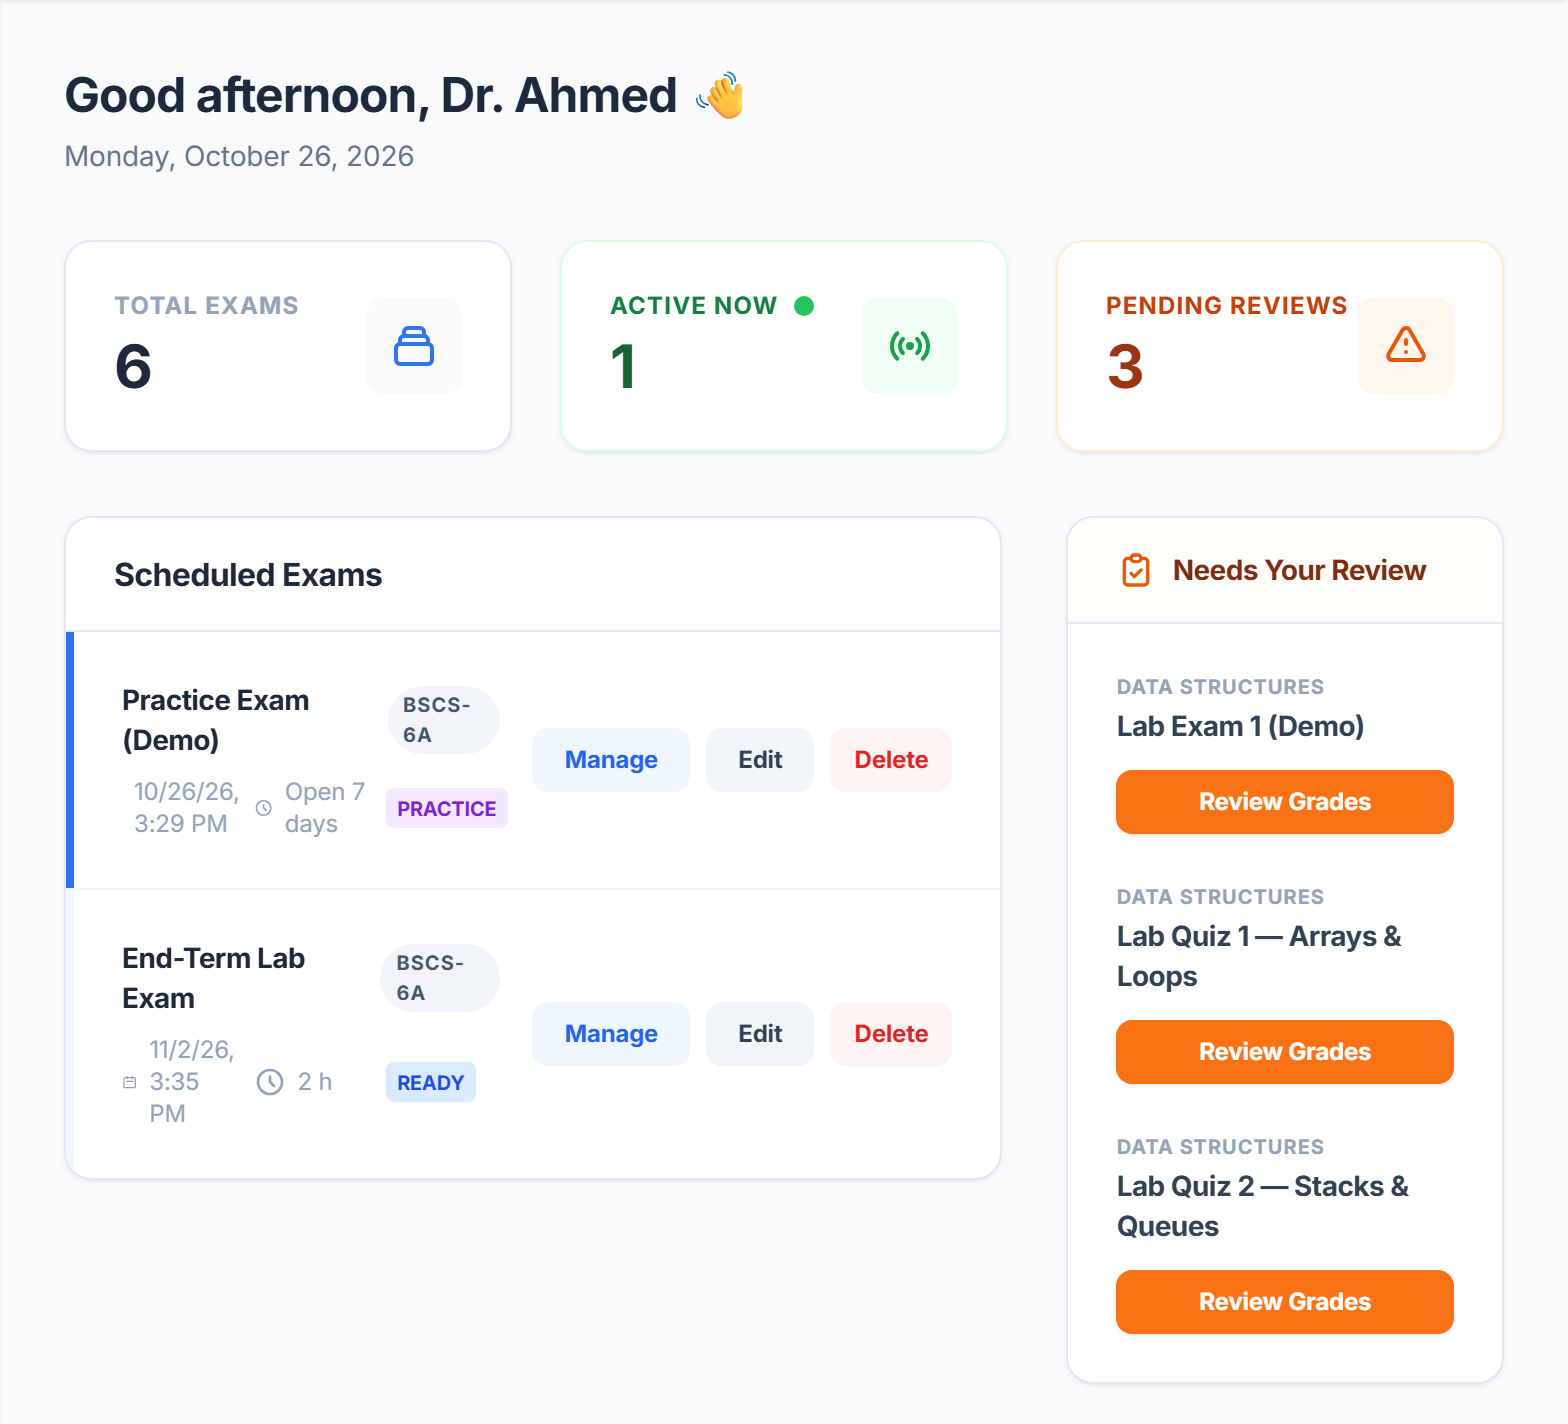
\includegraphics[width=\linewidth,height=410pt,keepaspectratio]{Figures/ui_teacher_dashboard.png}
\caption{Teacher Dashboard}
\label{fig:ui_teacher_dashboard}
\end{figure}
\SoftBarrierN

\begin{figure}[p]
\centering
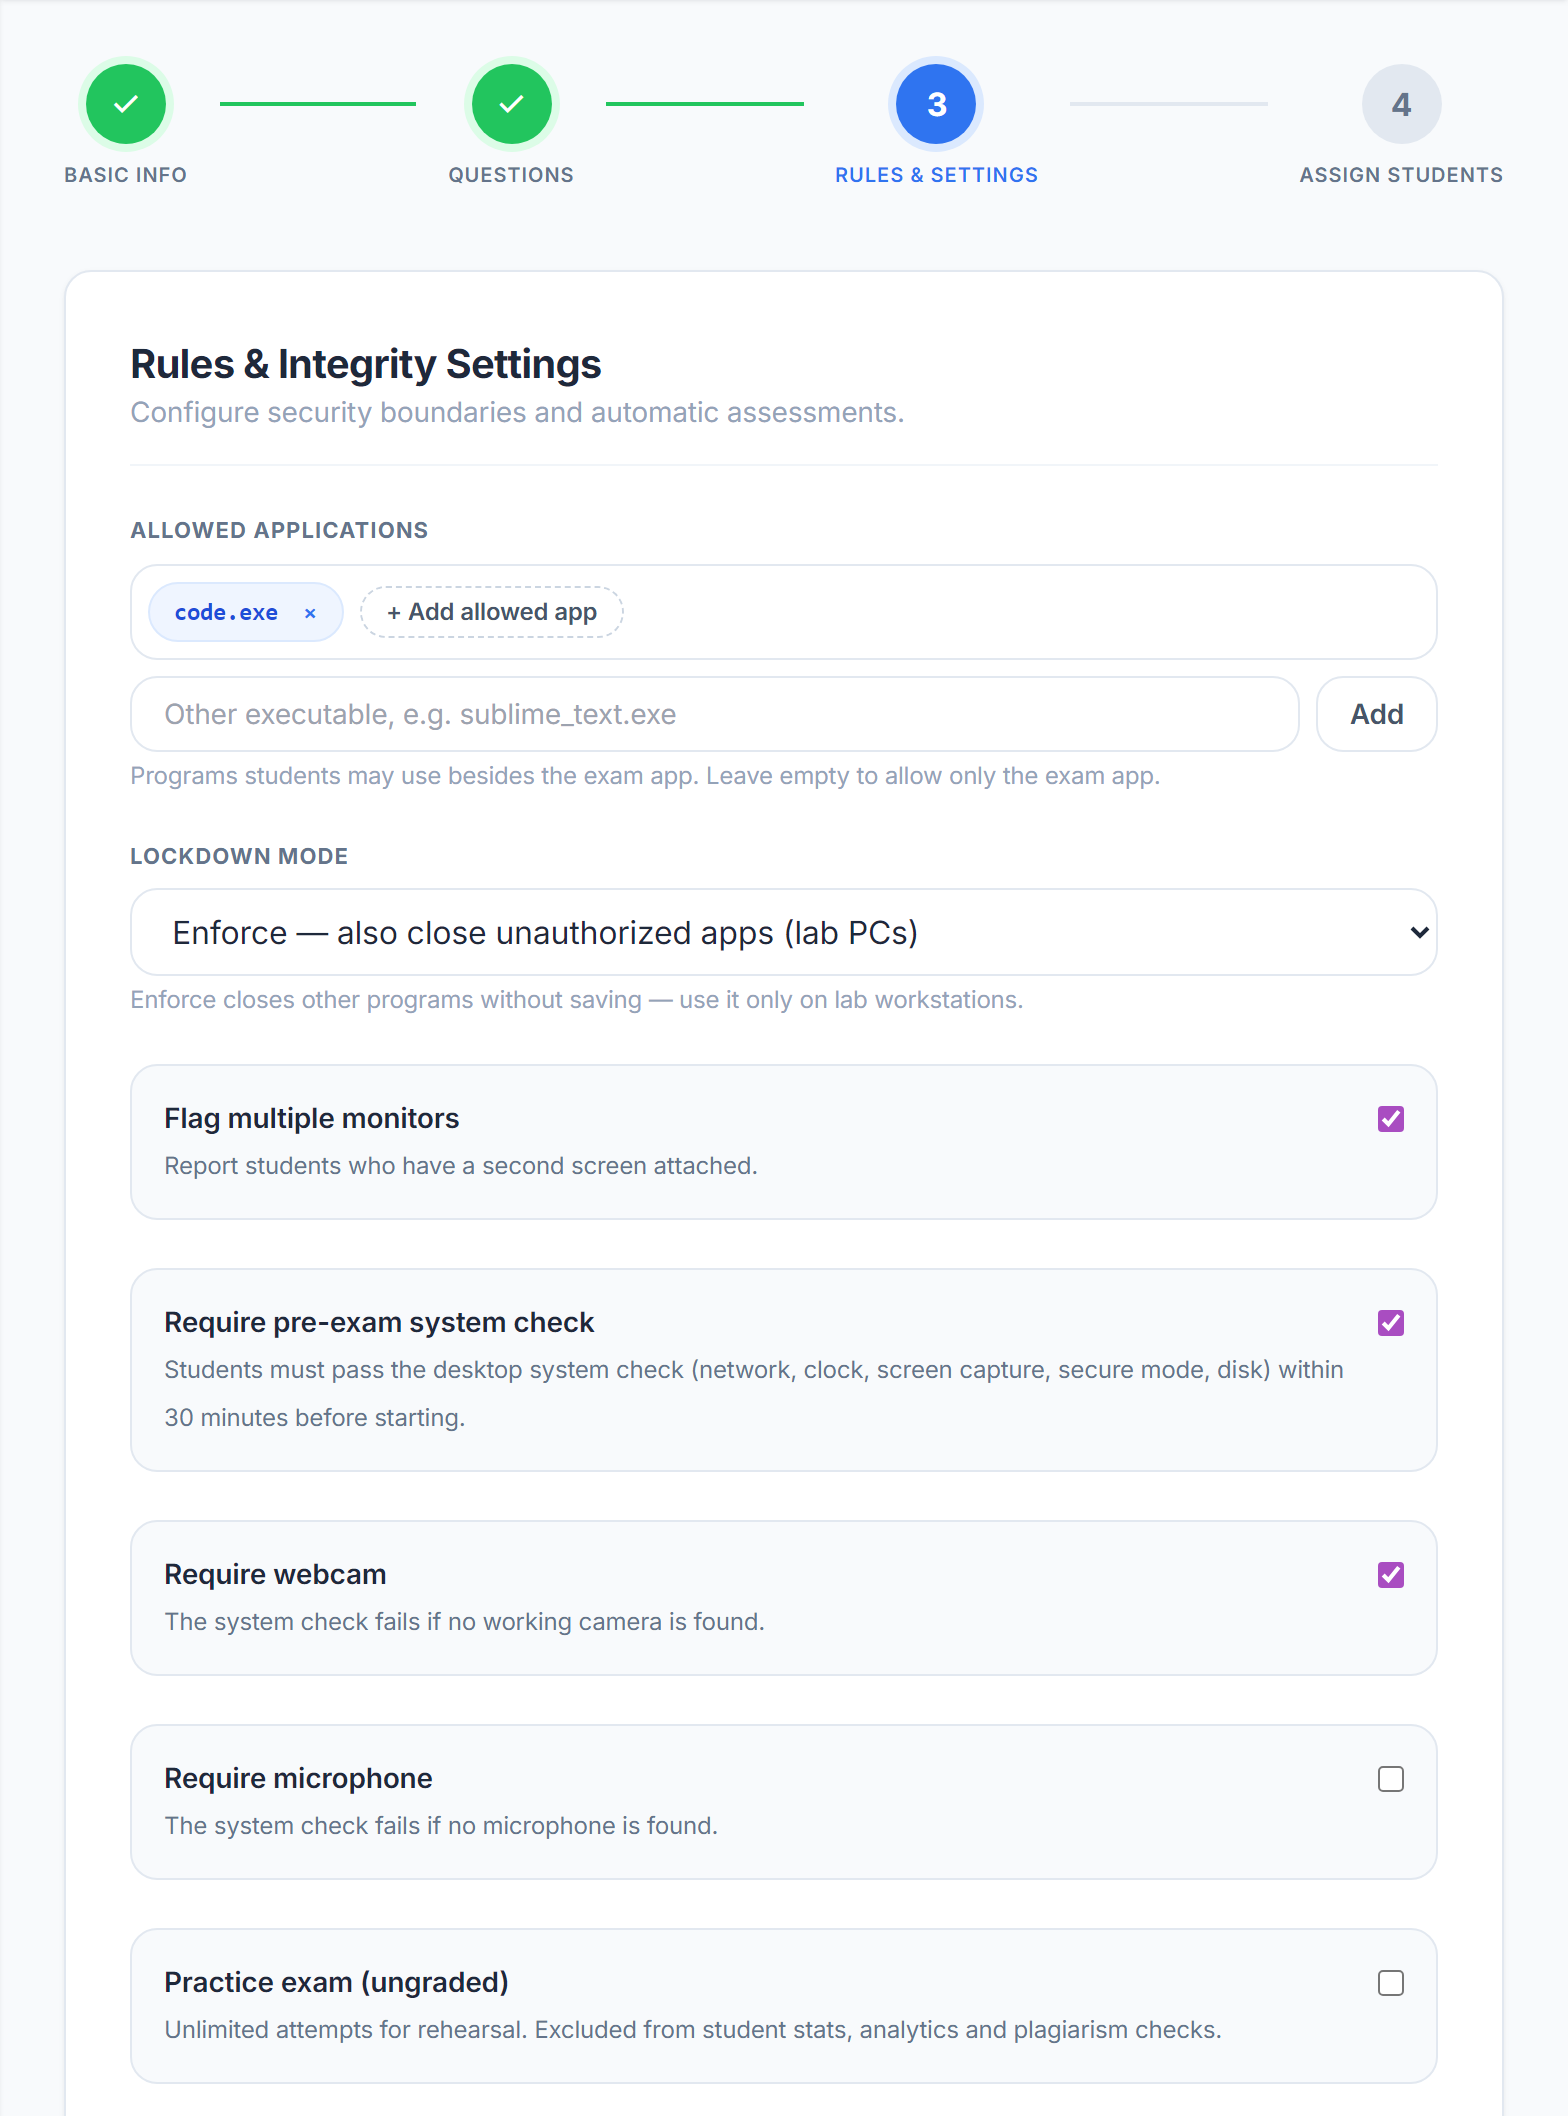
\includegraphics[width=\linewidth,height=628pt,keepaspectratio]{Figures/ui_create_exam_rules.png}
\caption{Create-Exam Wizard, Rules Step: Integrity Switches}
\label{fig:ui_create_exam_rules}
\end{figure}
\SoftBarrierN

A four-step wizard creates an exam: basic information, questions (MCQ, coding with test cases, theory), rules, and students (FR8). Step~3 holds the integrity rules: allowed applications, lockdown mode (Off, Report, Enforce), the multi-monitor flag, the required system check, webcam and microphone, and the practice-exam switch (Figure~\ref{fig:ui_create_exam_rules}); then early join, minimum attendance, the screenshot and webcam intervals, seat enforcement, AI evaluation and the plagiarism threshold (Figure~\ref{fig:ui_create_exam_rules_more}).

In Figure~\ref{fig:ui_create_exam_rules} the step bar shows that \emph{Basic Info} and \emph{Questions} are done and \emph{Rules \& Settings} is the current step. In this example only \texttt{code.exe} is allowed, and the lockdown mode is Enforce, which closes other programs without saving, so the hint says to use it only on lab PCs. The multi-monitor flag, the system check and the webcam are switched on, while the microphone and the practice-exam switch are off.

Figure~\ref{fig:ui_create_exam_rules_more} shows the lower half of the same step. Here early join is 0 minutes, the minimum attendance is 75\,\%, both capture intervals are 60~s, seat enforcement and AI evaluation are on, and the plagiarism threshold is 70\,\%. The hint under the screenshot interval explains that each gap is randomised by $\pm$50\,\% (30--90~s for 60~s) and that a violation causes an immediate capture, so a student cannot predict when the next capture comes.

\begin{figure}[tbp]
\centering
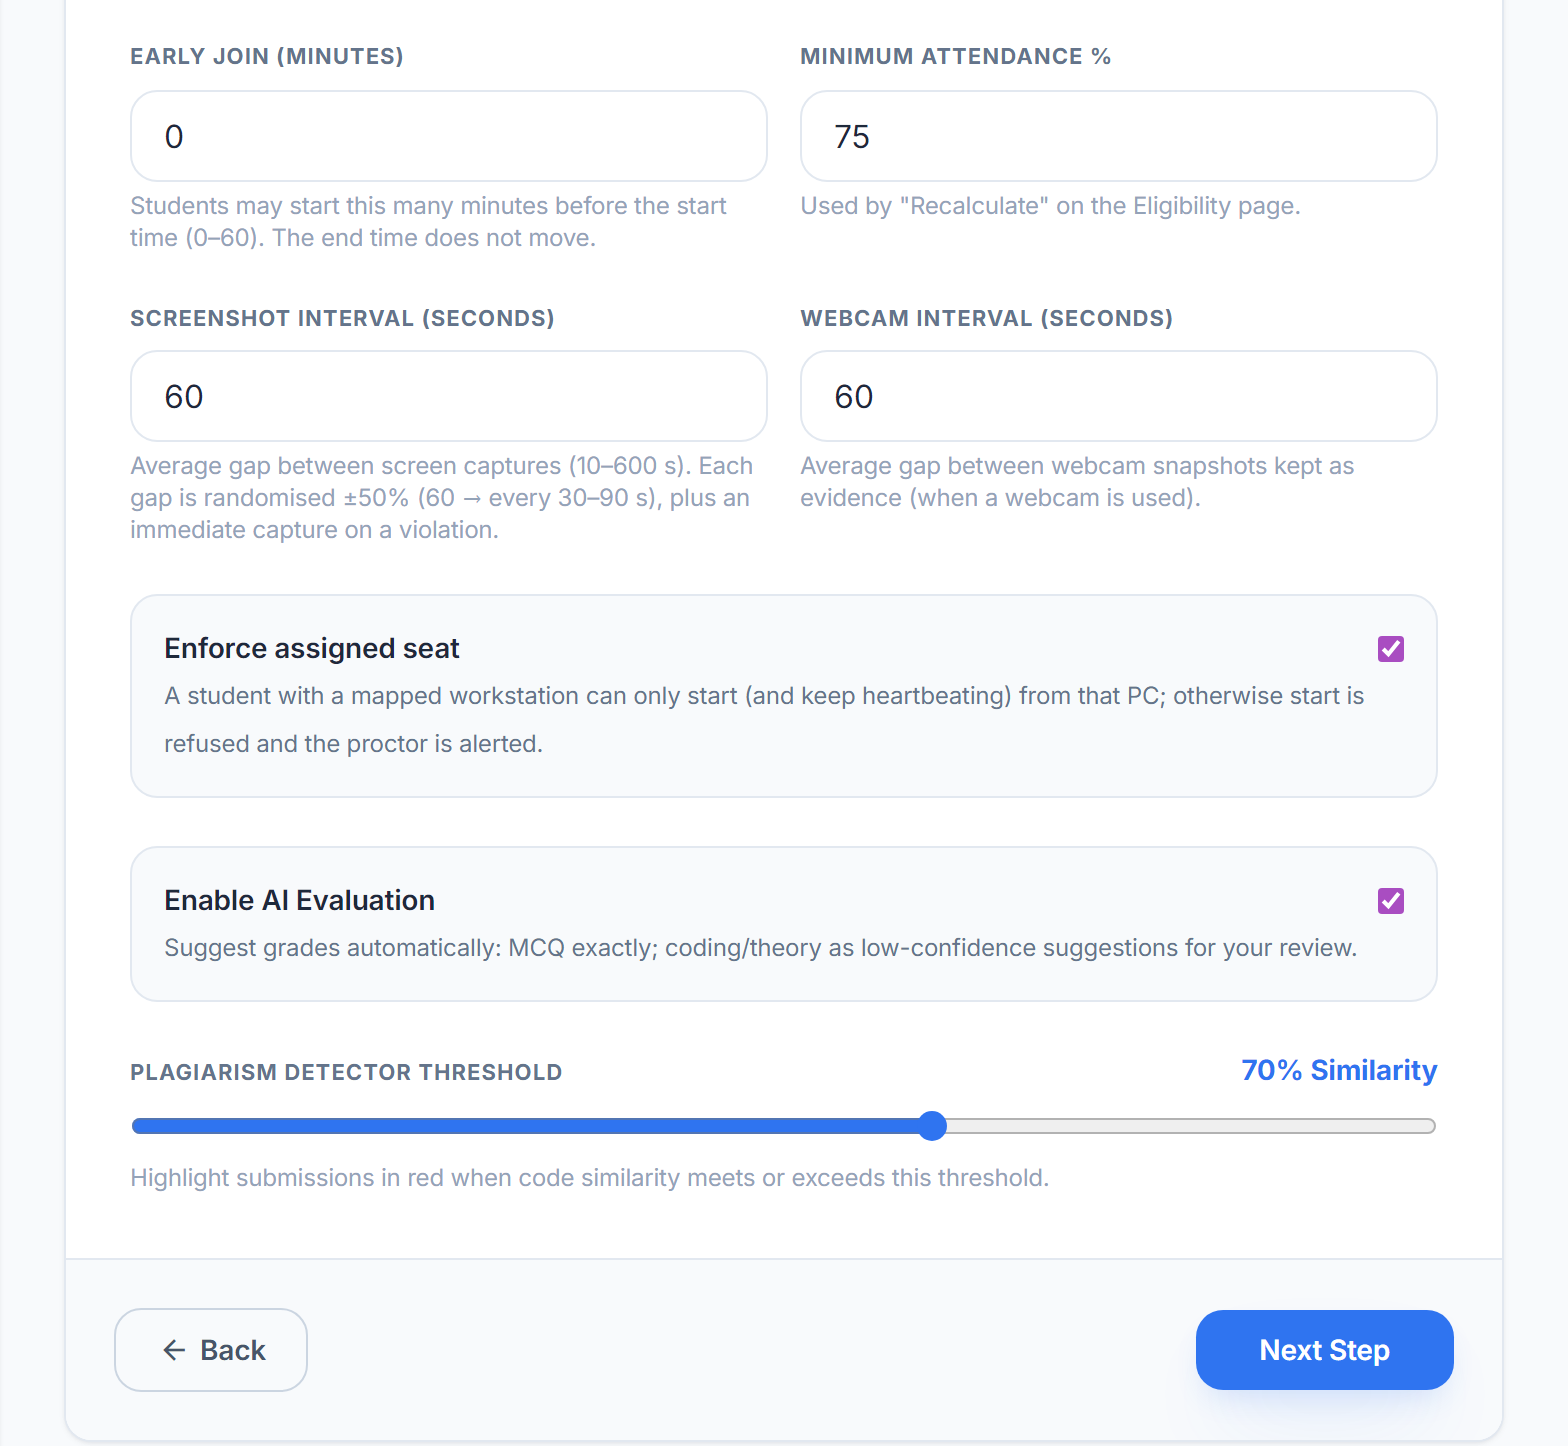
\includegraphics[width=\linewidth,height=416pt,keepaspectratio]{Figures/ui_create_exam_rules_more.png}
\caption{Create-Exam Wizard, Rules Step: Intervals, Seat, AI and Plagiarism Settings}
\label{fig:ui_create_exam_rules_more}
\end{figure}
\SoftBarrierN

On the eligibility page (Figure~\ref{fig:ui_eligibility}) the teacher uploads an attendance CSV (comma-separated values) file and clicks \emph{Recalculate}; students below the exam's minimum attendance become ineligible (FR9), as Hamza Iqbal (60\,\%) is here. Each row shows where its decision came from (\emph{Attendance} in the figure); a saved toggle for a single student becomes a \emph{Manual} override, which survives recalculation and is audited. The same page maps each student to a workstation (seat) and assigns invigilators, who then see only this exam.

The page is printed in two parts that show the same six rows in the same order. Part~(a) (Figure~\ref{fig:ui_eligibility}) holds the exam selector with its minimum attendance of 75\,\%, the \emph{Invigilators} card with Mr. Bilal assigned, and each student's name with a seat drop-down (R1C1 to R2C2 in Lab~A). Part~(b) (Figure~\ref{fig:ui_eligibility_b}) holds the buttons \emph{Upload Attendance}, \emph{Recalculate}, \emph{Mark All Eligible} and \emph{Mark All Ineligible}, the invigilator picker, and for each row the system check, the attendance, the eligibility switch with its source tag and the reason. Five students have 77.5--95\,\% attendance and are eligible. The last row is Hamza Iqbal: with 60\,\% (24 of 40 classes) his switch is off and the reason \emph{Attendance 60\% < 75\%} is shown in red. A green tick in the system-check column means a passing check less than 30 minutes old; Hamza has a dash because no check is recorded for him.

\begin{figure}[tbp]
\centering
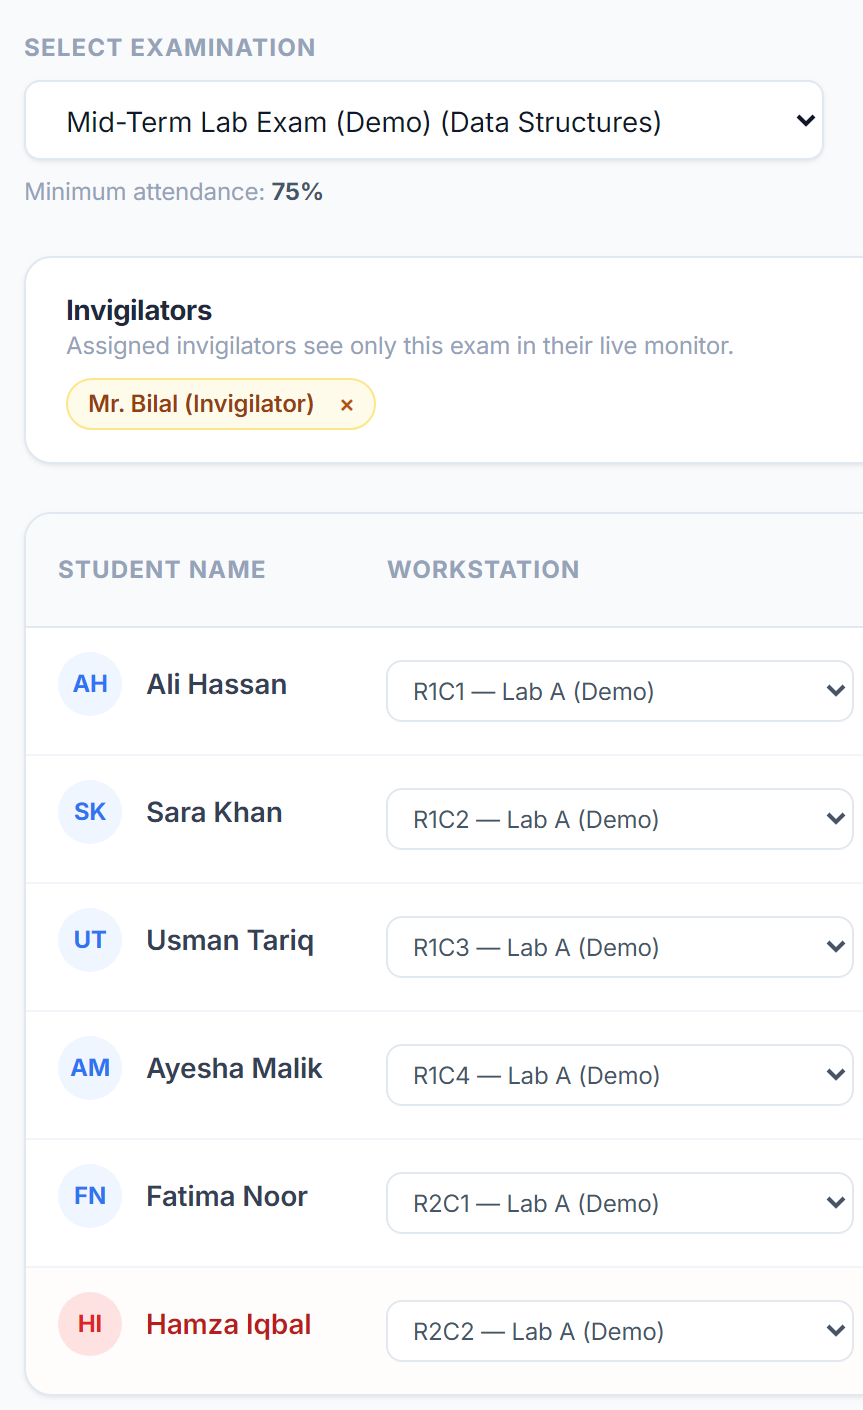
\includegraphics[width=0.72\linewidth]{Figures/ui_eligibility_p1.png}
\caption{Eligibility, Seats and Invigilators (a): Exam, Invigilators and Seats (Email Column Omitted)}
\label{fig:ui_eligibility}
\end{figure}
\SoftBarrierN

\begin{figure}[tbp]
\centering
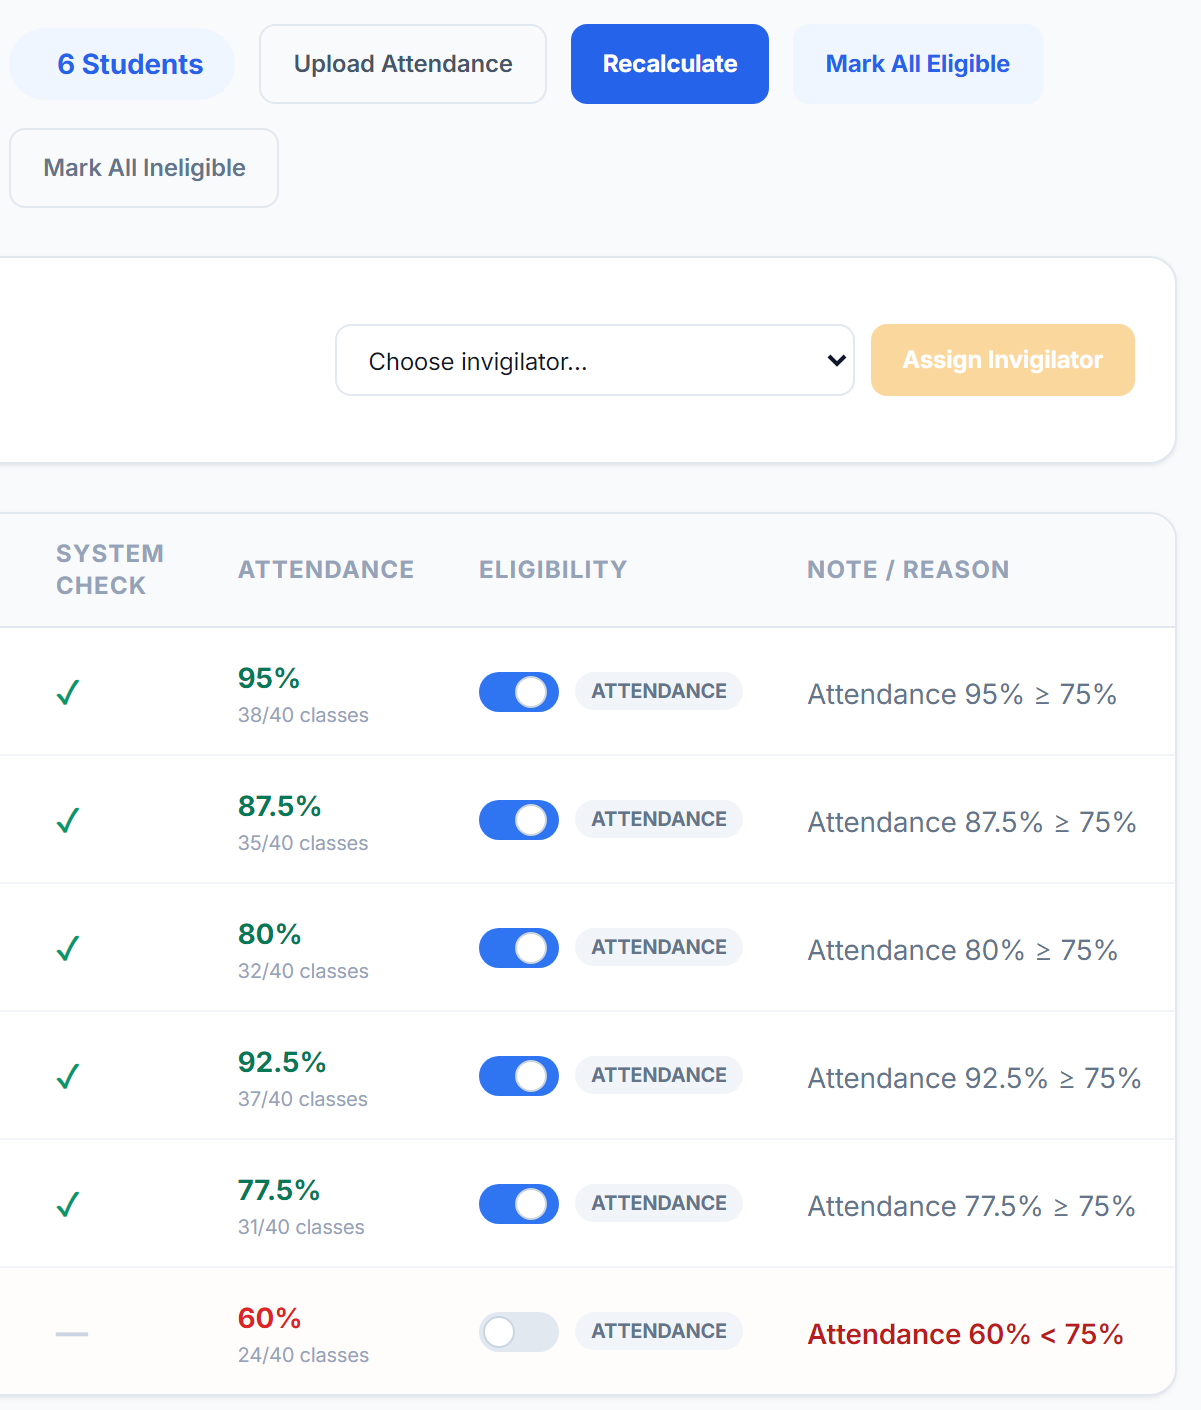
\includegraphics[width=\linewidth]{Figures/ui_eligibility_p2.png}
\caption{Eligibility, Seats and Invigilators (b): Attendance and Eligibility (Same Rows as Part (a))}
\label{fig:ui_eligibility_b}
\end{figure}
\SoftBarrierN

\subsection{Live Invigilation}\suppressfloats[t]
SignalR carries live updates between the API and the web dashboard; the desktop client uses REST only and receives invigilator warnings, extra time, unlocks and force-submits in the reply to its next heartbeat (every 10~s). The client sends heartbeats, event batches and screen captures to \url{/api/monitoring}, and the server pushes each update to the live monitor (Figures~\ref{fig:ui_teacher_live_monitoring} to~\ref{fig:ui_teacher_live_monitoring_b}) over the hub \url{/hubs/monitoring} (FR5, FR10). Through \texttt{ExamProctors}, invigilators see only the exams assigned to them. The header of the live monitor (Figure~\ref{fig:ui_teacher_live_monitoring}) names the current exam with its course tag and an exam selector, and shows the remaining time (01:27:10) on the right. It also shows that four students are still sitting (Ali Hassan has already submitted) and gives the \emph{Extend Time} and \emph{Force End Exam} buttons, which act on the whole exam.

\begin{figure}[tbp]
\centering
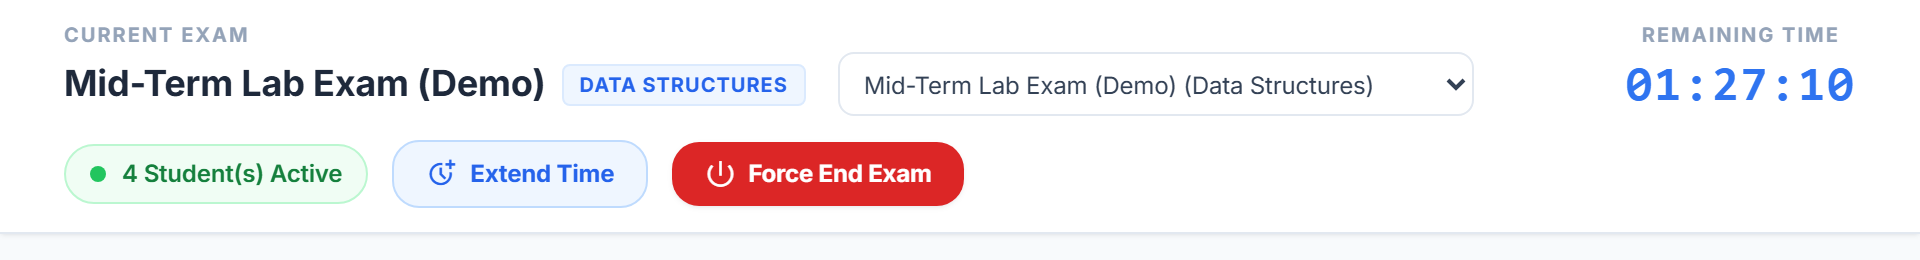
\includegraphics[width=\linewidth]{Figures/ui_live_monitor_a_p1.png}
\caption{Live Monitor (a): Header with Remaining Time and Exam Controls}
\label{fig:ui_teacher_live_monitoring}
\end{figure}
\SoftBarrierN

Below the header each student has a tile (Figures~\ref{fig:ui_teacher_live_monitoring_tiles} to~\ref{fig:ui_teacher_live_monitoring_b}). Each tile shows the student's seat and PC with the Windows user, readiness, latest capture, latest alert and progress as answered questions with a bar. The heart icon and the border colour give the status: the classifier level as Stable (Normal), Warning, Suspicious or Critical (Violation); a client silent for 30~s is shown as Disconnected, and a finished session as Submitted, Force submitted or Timed out. The captures are small thumbnails, and their text is not meant to be read at this size.

Ali Hassan (seat R1C1) has answered all three questions and submitted, and Sara Khan (R1C2) is a Warning with one alert, \emph{Blocked keys}, for her blocked Alt+Tab (Figure~\ref{fig:ui_teacher_live_monitoring_tiles}). Usman Tariq (R1C3) is Critical with two alerts and one incident (Figure~\ref{fig:ui_teacher_live_monitoring_tile3}): he opened Chrome, which is not on the allowed list, and Enforce mode closed it, as the line \emph{Unauthorized app closed: chrome (Killed)} says; his capture shows a browser search. In the second row (Figure~\ref{fig:ui_teacher_live_monitoring_b}), Ayesha Malik's phone in view makes her Suspicious, and Fatima Noor is Stable with an \emph{Idle 9m} badge, which means no keyboard or mouse input on her PC for nine minutes.

\begin{figure}[tbp]
\centering
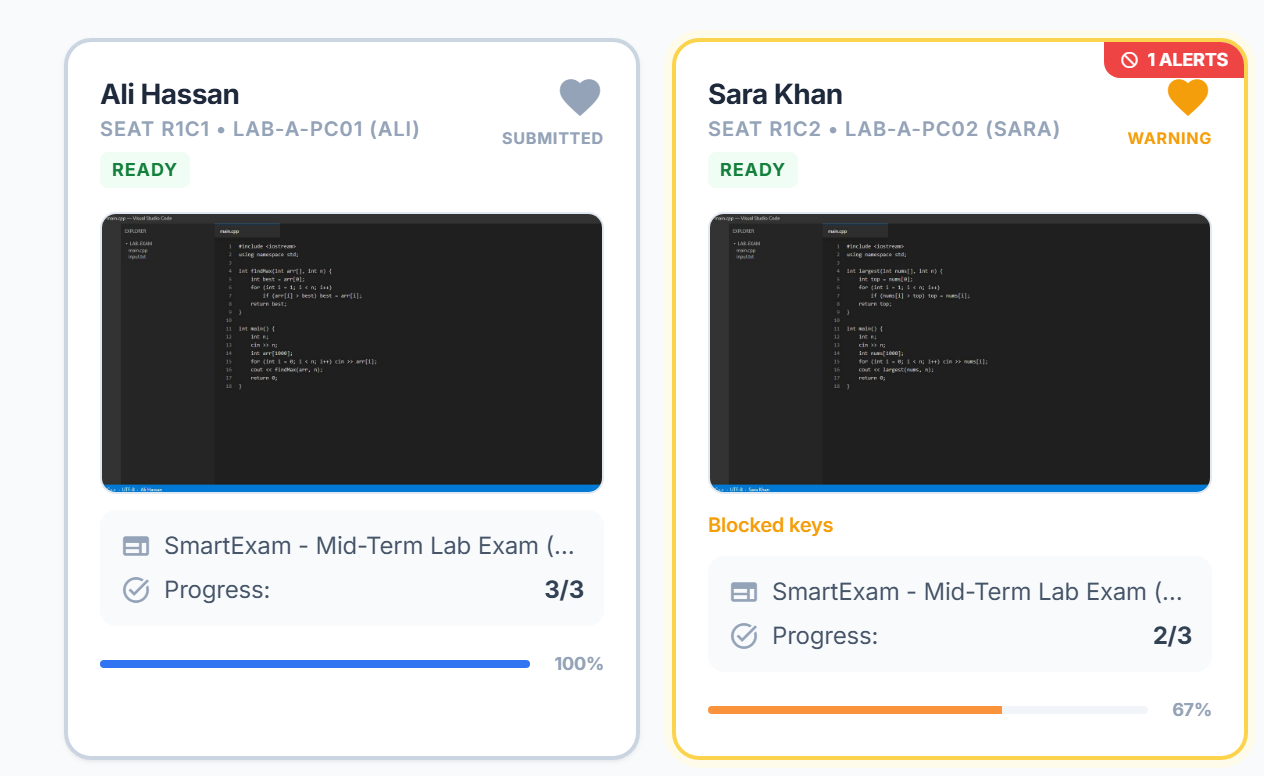
\includegraphics[width=\linewidth]{Figures/ui_live_monitor_a_p2.png}
\caption{Live Monitor (b): First Row, Tiles of Ali Hassan and Sara Khan}
\label{fig:ui_teacher_live_monitoring_tiles}
\end{figure}
\SoftBarrierN

\begin{figure}[tbp]
\centering
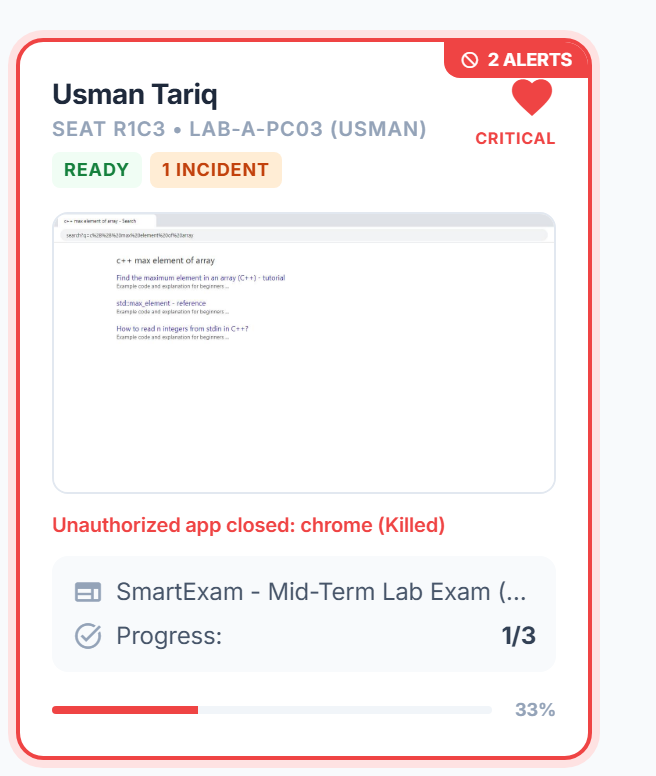
\includegraphics[width=0.52\linewidth]{Figures/ui_live_monitor_a_p3.png}
\caption{Live Monitor (c): First Row, Tile of Usman Tariq}
\label{fig:ui_teacher_live_monitoring_tile3}
\end{figure}
\SoftBarrierN

\begin{figure}[tbp]
\centering
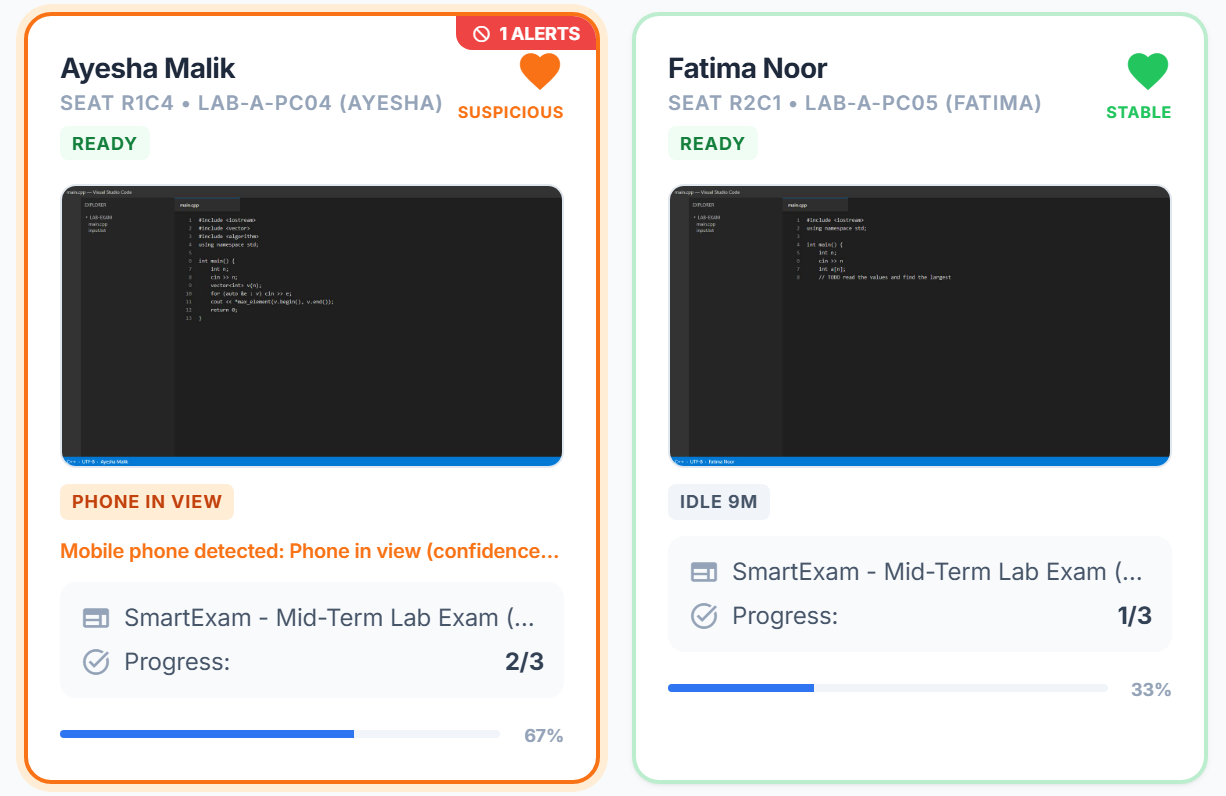
\includegraphics[width=\linewidth,height=293pt,keepaspectratio]{Figures/ui_live_monitor_b.png}
\caption{Live Monitor (d): Second Row of Tiles}
\label{fig:ui_teacher_live_monitoring_b}
\end{figure}
\SoftBarrierN

Clicking a tile opens the student drawer, here for Usman Tariq (Figure~\ref{fig:ui_live_drawer}). Its top gives the seat, the PC and the Windows user with the number of active alerts and open incidents. Below are the latest captures (the newer one, outlined in orange, shows the browser search), the readiness result (all seven checks passed on LAB-A-PC03 at 3:35:26~PM) and the applications seen on the PC, where Chrome is struck through because it is no longer running. So the invigilator sees all the evidence for one student in one place before acting.

\begin{figure}[p]
\centering
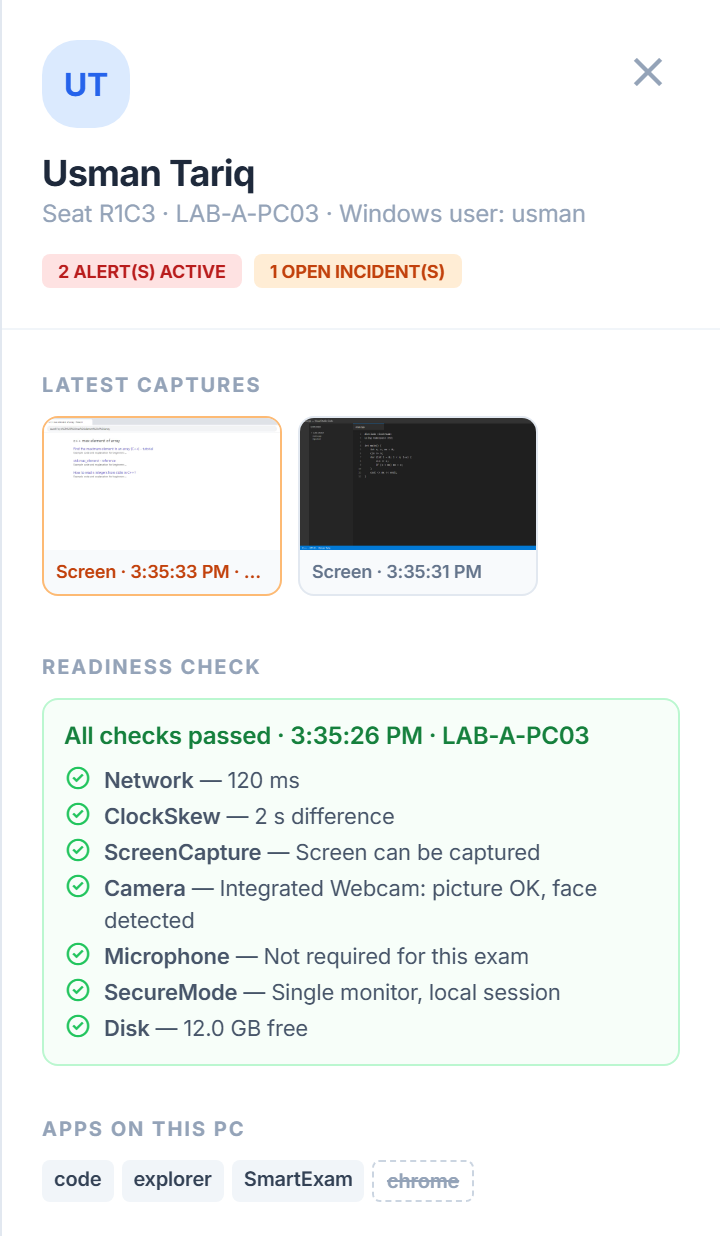
\includegraphics[width=\linewidth,height=628pt,keepaspectratio]{Figures/ui_live_drawer_evidence.png}
\caption{Student Drawer (a): Evidence}
\label{fig:ui_live_drawer}
\end{figure}
\SoftBarrierN

From the action panel (Figure~\ref{fig:ui_live_drawer_b}) the invigilator sends a warning, records an incident, unlocks the PC for five minutes with a short reason (the server allows 1--30 minutes), grants extra time or force-submits the session (FR10). The green line \emph{Warning Message Sent} confirms that the warning was sent. Force-submit is the red button because it ends the student's attempt; like the other actions, it reaches the desktop client in the reply to its next heartbeat.

\begin{figure}[tbp]
\centering
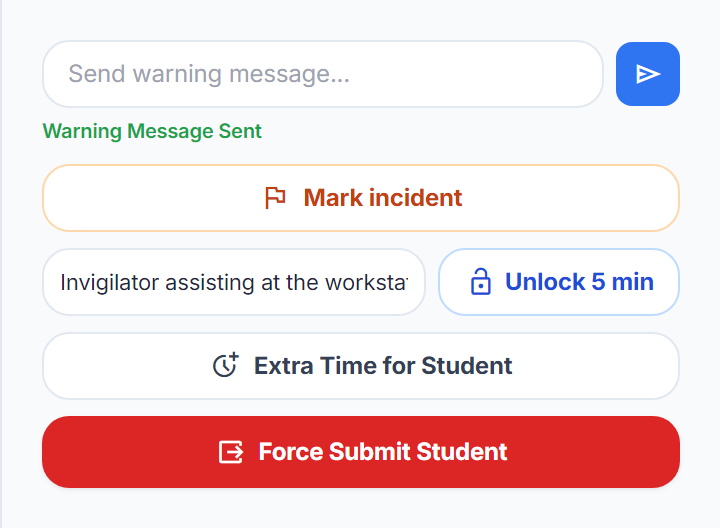
\includegraphics[width=0.55\linewidth]{Figures/ui_live_drawer_actions.png}
\caption{Student Drawer (b): Actions}
\label{fig:ui_live_drawer_b}
\end{figure}
\SoftBarrierN

Further down (Figure~\ref{fig:ui_live_timeline}) are the open incidents, with \emph{Escalate} and \emph{Mark resolved}, and the activity timeline. The incident card shows its severity (High), its status (Open), the note and who recorded it (Dr. Ahmed). The timeline lists the events newest first: Chrome closed by Enforce mode at 3:35:33~PM, the incident recorded at the same time, and the warning sent ten seconds later, which is the banner of Figure~\ref{fig:ui_student_warning}.

\begin{figure}[tbp]
\centering
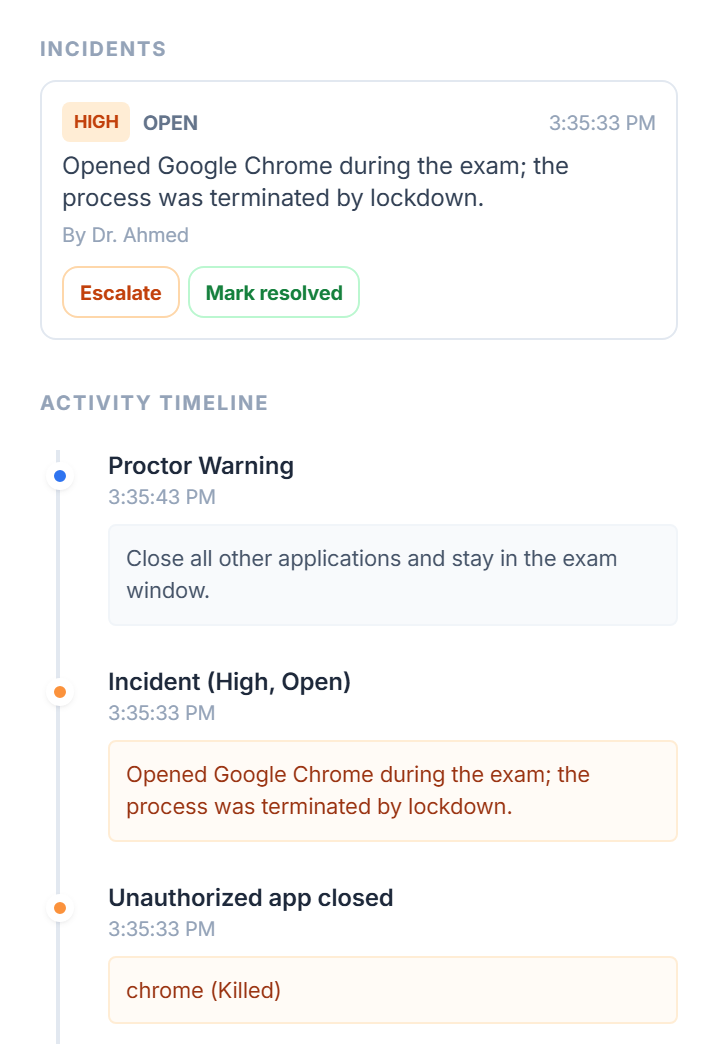
\includegraphics[width=0.60\linewidth,height=418pt,keepaspectratio]{Figures/ui_live_timeline.png}
\caption{Student Drawer (c): Incident and Activity Timeline}
\label{fig:ui_live_timeline}
\end{figure}
\SoftBarrierN

\subsection{Evaluation}\suppressfloats[t]
The results page lists each submission with its score and SHA-256 receipt. Opening one (Figures~\ref{fig:ui_teacher_ai_grading} and~\ref{fig:ui_teacher_ai_grading_b}) shows every answer next to its AI evaluation: suggested mark, confidence, engine, justification, test-case results (hidden cases marked) and code-analysis signals. Coding answers (C or C++ only) are compiled and run against weighted test cases \cite{alamutka2005} in an isolated Docker \texttt{gcc:13} container when Docker is available; otherwise a local MinGW g++ runner, which is not isolated, is used, and with no runner the answer is left for teacher review (FR11.1). Theory answers get a TF-IDF similarity score \cite{salton1988} (FR11.2). The teacher accepts the mark or saves an override, stored in \texttt{TeacherGradeOverrides}.

Figure~\ref{fig:ui_teacher_ai_grading} shows the top of the review for Usman Tariq: his status (Submitted), the question with its type and maximum (Coding, 20 marks) and his submitted code. His program starts the maximum at 0 instead of at the first element, so it prints a wrong answer when all the numbers are negative. The evaluation card below shows how the grader finds this mistake.

\begin{figure}[tbp]
\centering
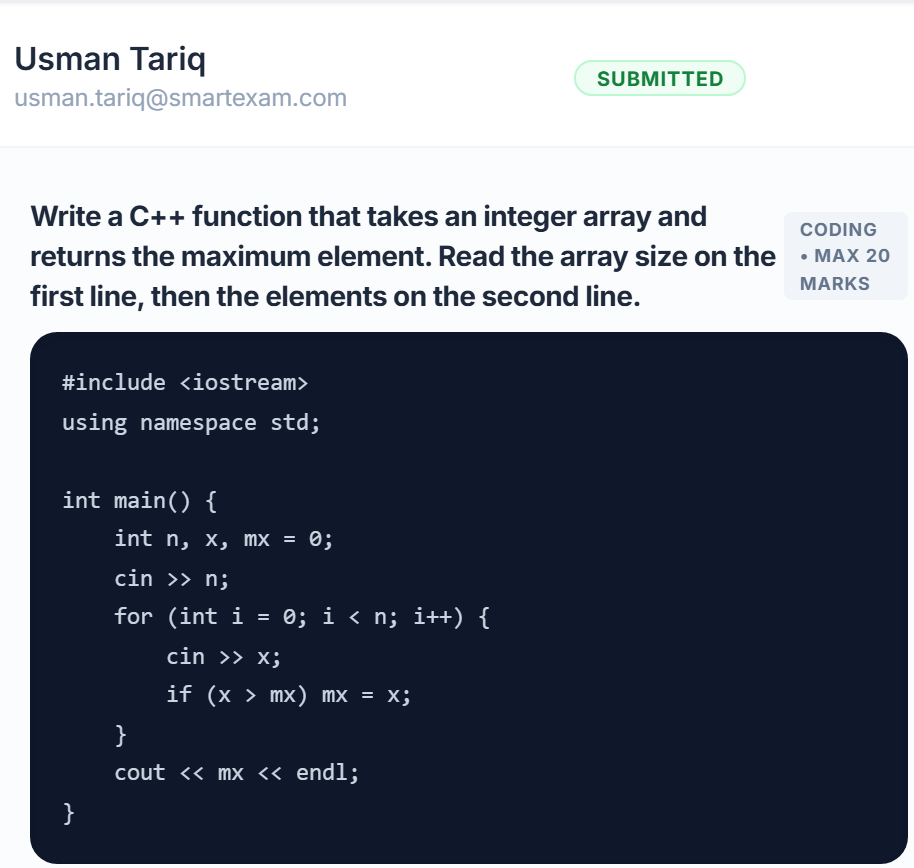
\includegraphics[width=0.85\linewidth,height=370pt,keepaspectratio]{Figures/ui_ai_grading_answer.png}
\caption{AI Evaluation of a Coding Answer (a): Question and Submitted Code}
\label{fig:ui_teacher_ai_grading}
\end{figure}
\SoftBarrierN

The AI evaluation card (Figure~\ref{fig:ui_teacher_ai_grading_b}) suggests 10 of 20 marks with medium confidence, from the isolated Docker engine. The test-case table explains the mark: the visible case passes, but the hidden case with the input $-1$, $-5$, $-2$ expects $-1$ and gets 0, so one of the two cases passes and half the marks are suggested. The code-analysis signals give O($n$) complexity, one loop and a medium hard-coding suspicion, because the code passes every visible case but fails a hidden one. The teacher can accept the 10 marks or enter another mark with a note and click \emph{Save Grade Override}.

\begin{figure}[tbp]
\centering
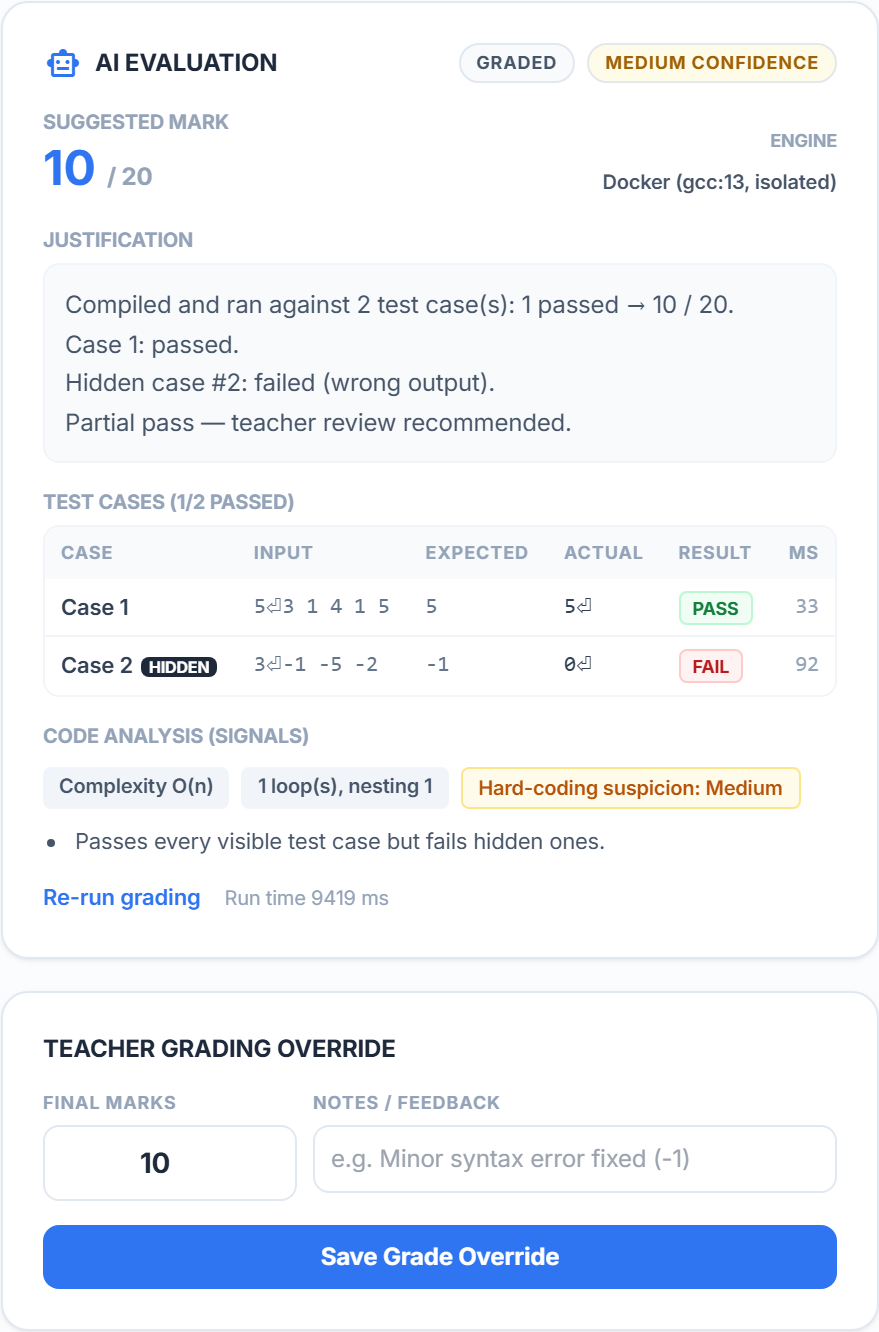
\includegraphics[width=\linewidth,height=565pt,keepaspectratio]{Figures/ui_ai_grading_eval.png}
\caption{AI Evaluation of a Coding Answer (b): Suggested Mark, Test Cases and Override}
\label{fig:ui_teacher_ai_grading_b}
\end{figure}
\SoftBarrierN

The \emph{Plagiarism Flags} tab (Figure~\ref{fig:ui_plagiarism}) shows a pairwise heat map built by k-gram winnowing \cite{winnowing}, which ignores identifiers and comments in code (FR11.3). A pair at or above the exam's threshold gets a card with both answers side by side and the matched lines highlighted; here Sara's program is Ali's with renamed variables. The teacher records the decision as a grade override.

In the heat map each row and column is a student (the columns use initials), and each cell is the highest similarity of that pair over all questions; darker cells are more similar, in 20\,\% steps. Only Ali Hassan and Sara Khan reach the 70\,\% threshold, at 100\,\%, while every other pair is at 25\,\% or below. The card below shows why: only the names differ (\texttt{largest}, \texttt{nums}, \texttt{top} against \texttt{findMax}, \texttt{arr}, \texttt{best}), so with identifiers ignored the code is the same. A note at the bottom reminds the teacher that similarity is evidence, not a verdict.

\begin{figure}[p]
\centering
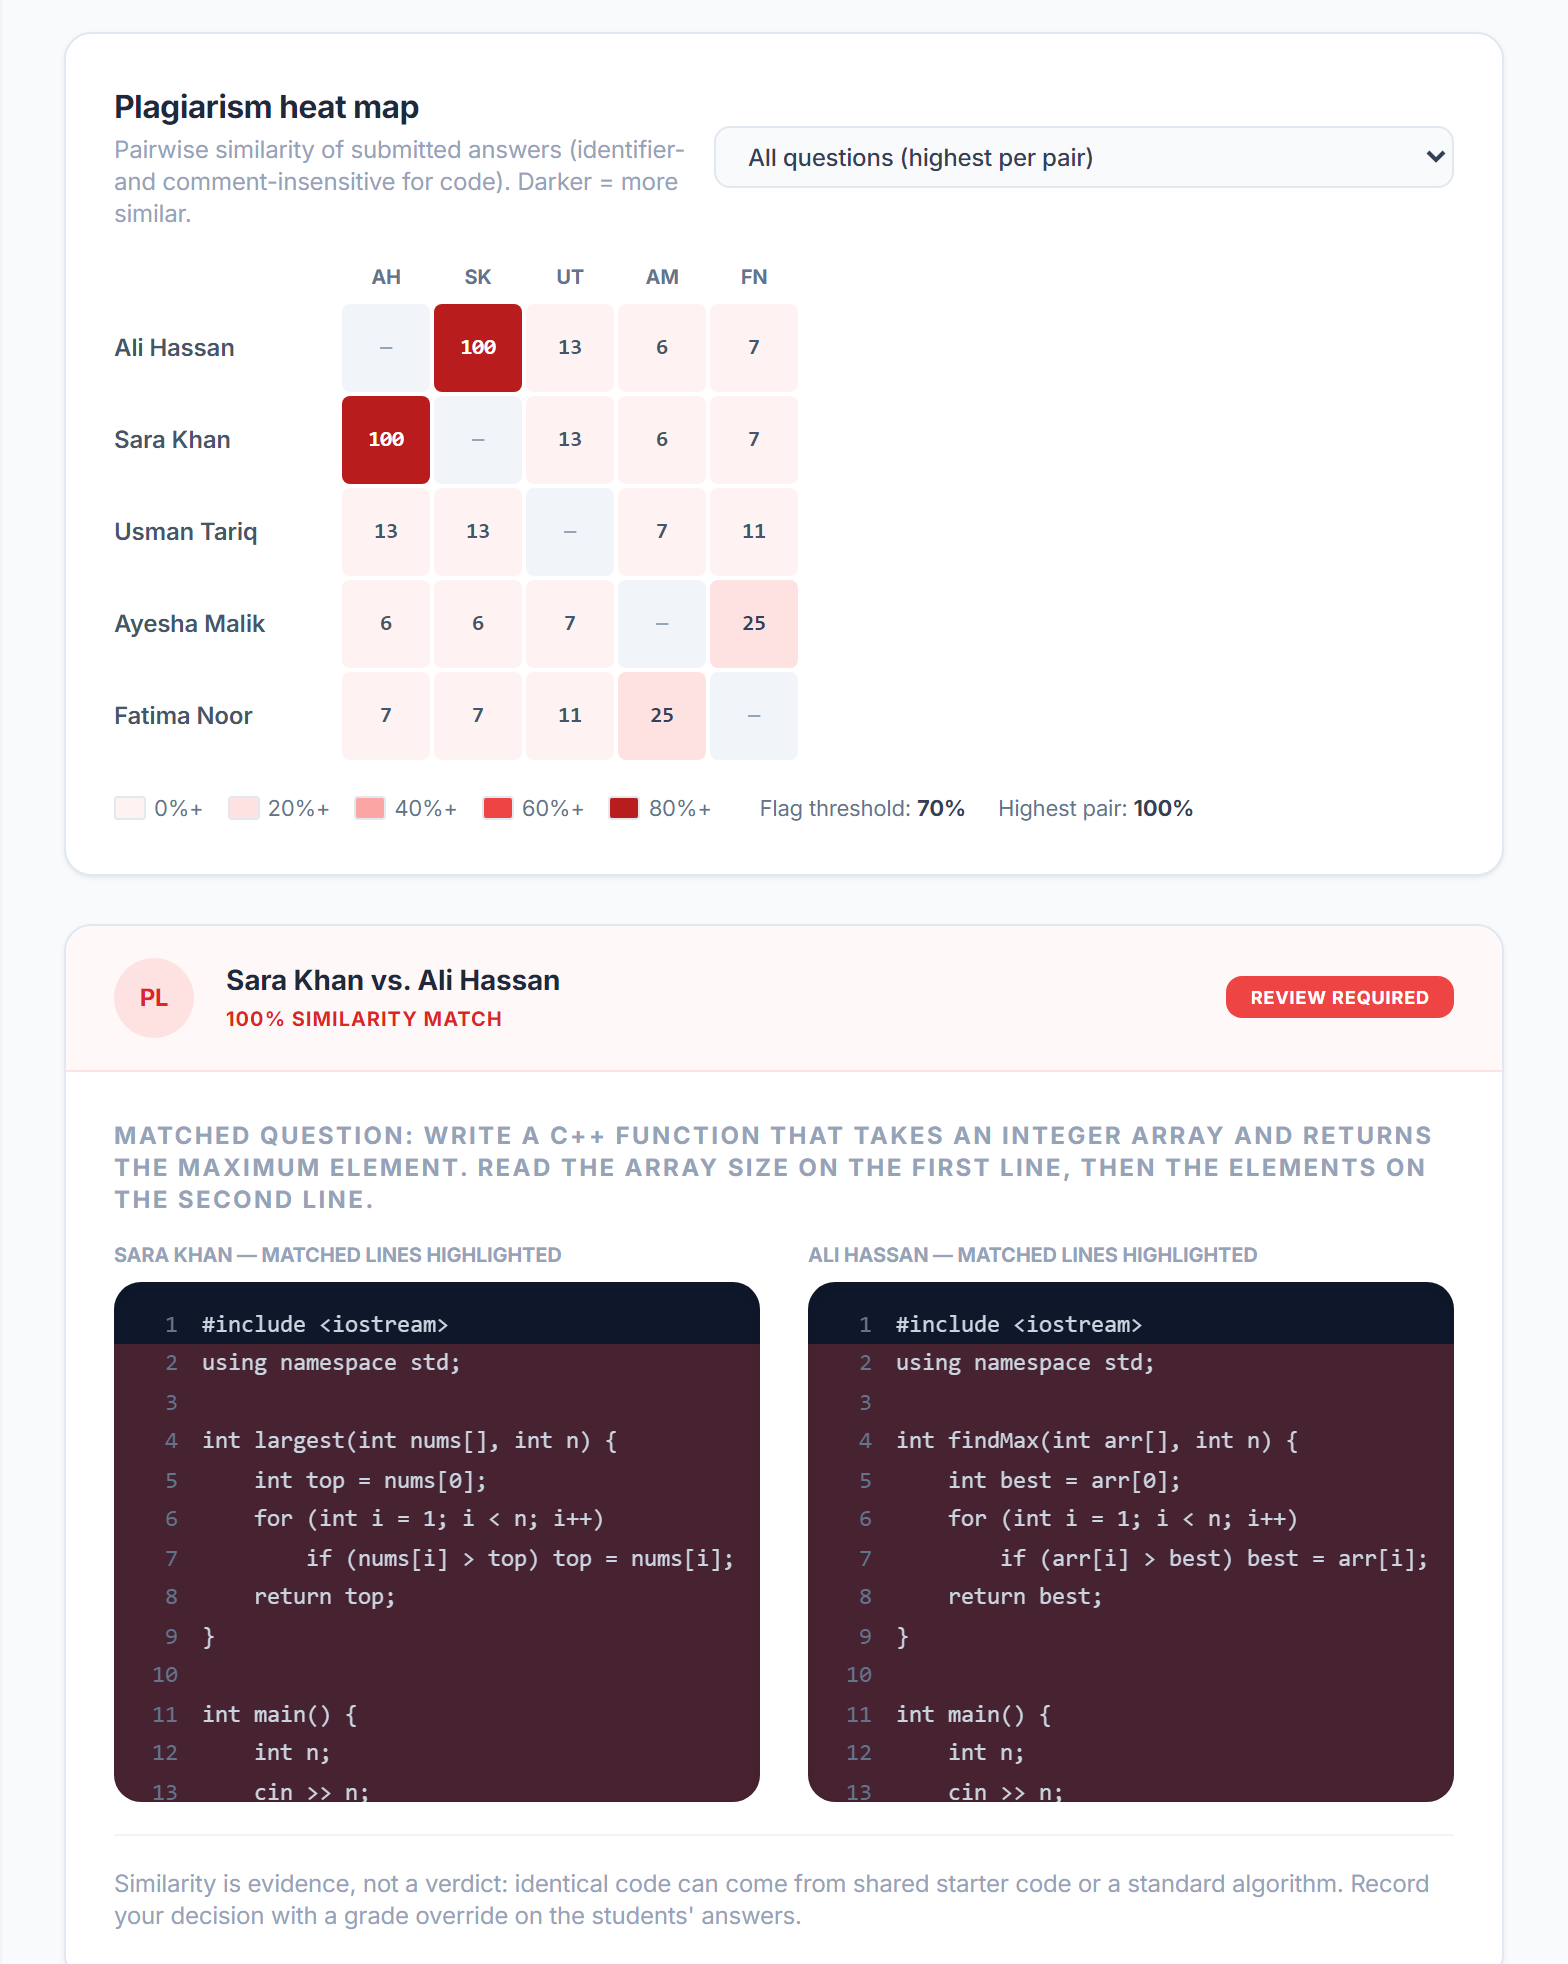
\includegraphics[width=\linewidth,height=562pt,keepaspectratio]{Figures/ui_plagiarism.png}
\caption{Plagiarism Heat Map and Matched Pair}
\label{fig:ui_plagiarism}
\end{figure}
\SoftBarrierN

\subsection{Administration and Student Portal}\suppressfloats[t]
Every web user, staff or student, signs in on one login page with email and password (Figure~\ref{fig:ui_web_login}) and is taken to the home page of their role. Neither front end offers self-registration or an emailed password reset: administrators create accounts or import them from a CSV file and can set a new password when editing an account (FR7), and staff change their own password from the panel (Figure~\ref{fig:seq_change_password}). The desktop client's sign-in and logout are drawn in Figures~\ref{fig:seq_login} and~\ref{fig:seq_logout}; on the web panel, sign-in, refresh and sign-out are tested in ST-01 (Table~\ref{tab:st_admin}). The figure shows the form filled in for the teacher account (\texttt{teacher@smartexam.com}), with an eye icon to show or hide the password. The note under \emph{Sign In} says that access attempts are logged, and this is true: the server writes every successful and failed login to the audit log (\texttt{LOGIN\_SUCCESS}, \texttt{LOGIN\_FAILED}).

\begin{figure}[htbp]
\centering
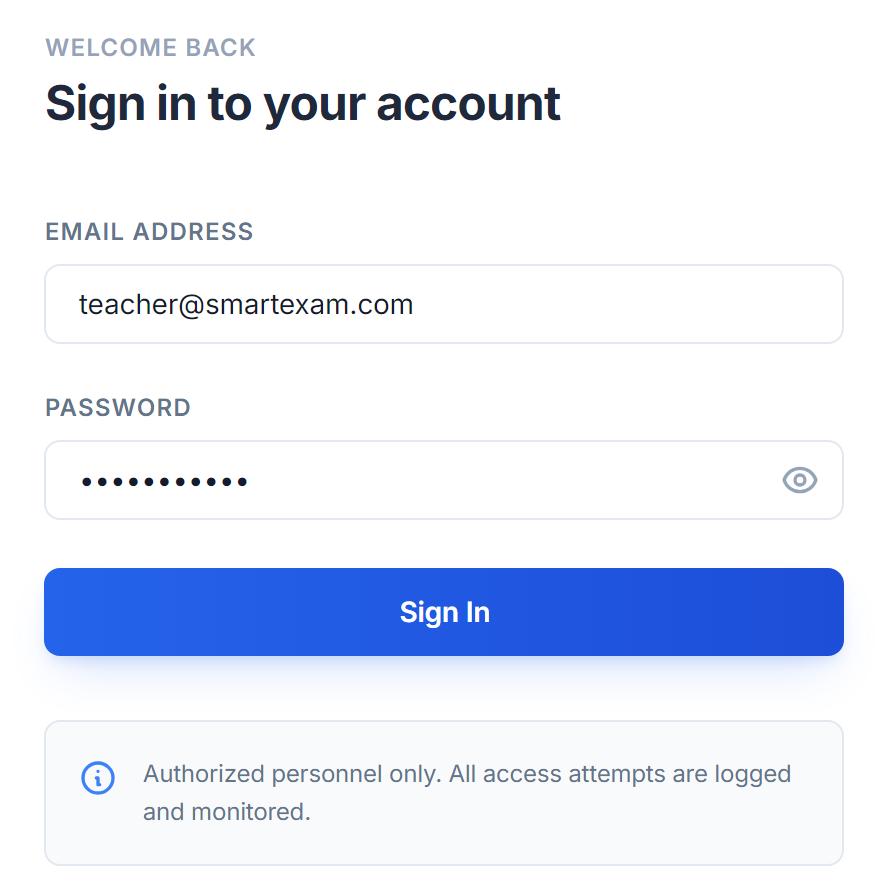
\includegraphics[width=0.62\linewidth]{Figures/ui_web_login.png}
\caption{Web Panel Login (Sign-In Form)}
\label{fig:ui_web_login}
\end{figure}
\SoftBarrierN

Admins manage departments and courses (Figure~\ref{fig:ui_academics}); department names are unique, a course code is unique within its department, and a department or course still in use cannot be deleted (FR7). The upper card lists the three departments with their number of courses (Computer Science 3, Electrical Engineering 1, Software Engineering 2). The lower card lists the six courses with code, name, department and number of sections, and can be filtered by department. Only CS301 Data Structures has a section, the one that owns the demo exams, so it is the only course here that cannot be deleted.

\begin{figure}[tbp]
\centering
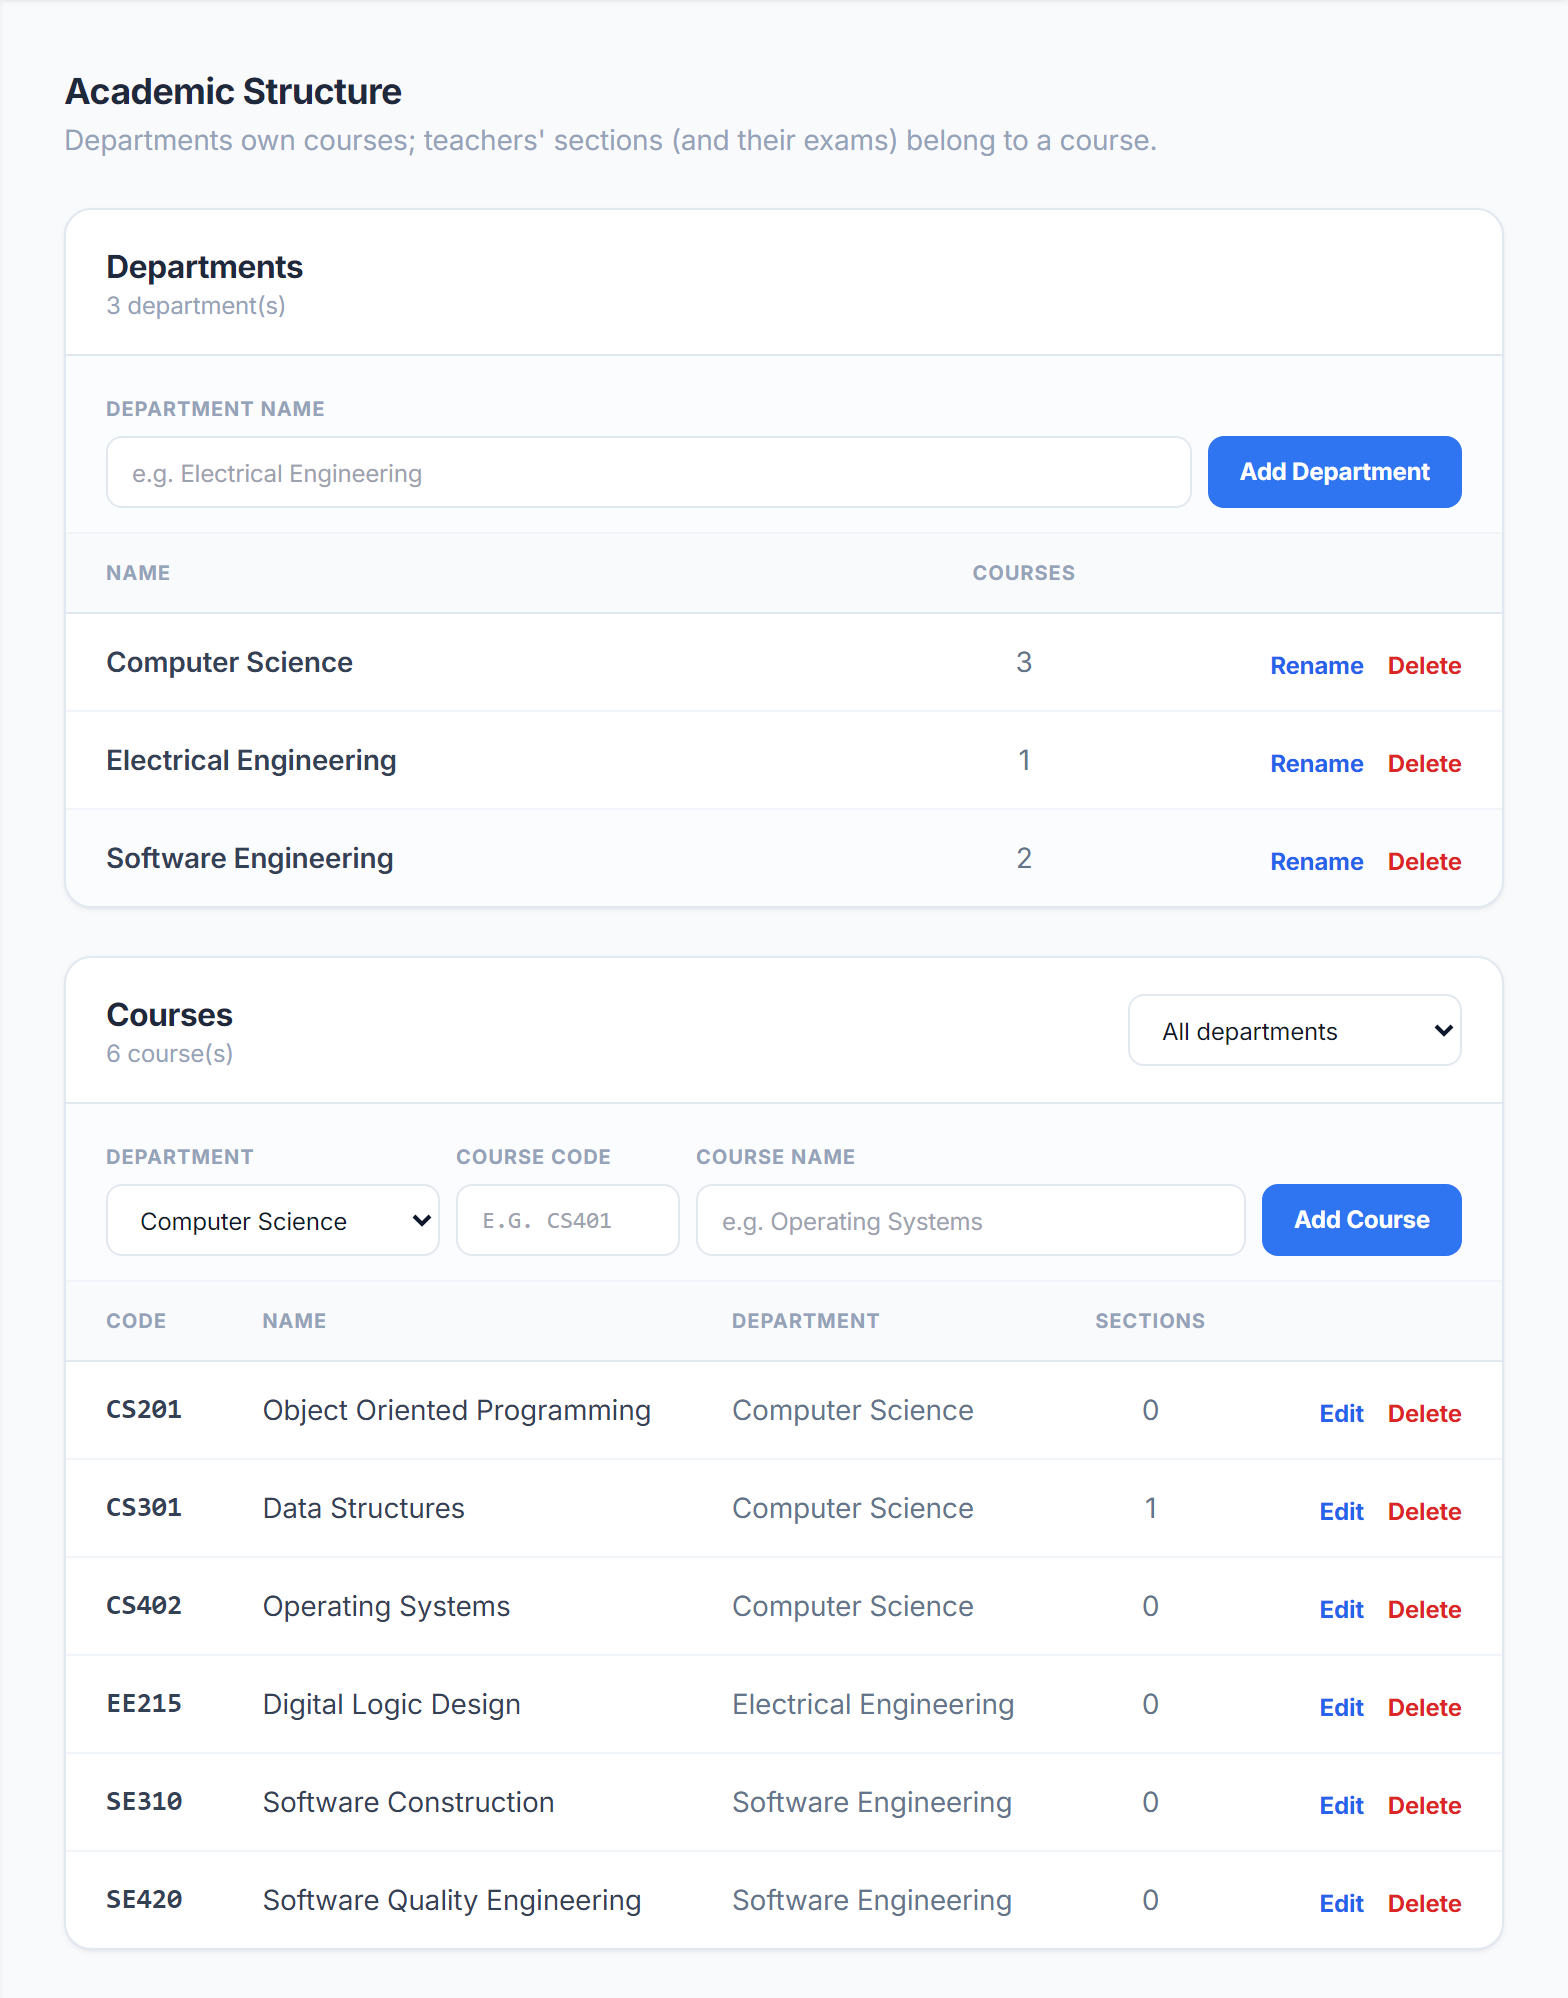
\includegraphics[width=\linewidth,height=600pt,keepaspectratio]{Figures/ui_academics.png}
\caption{Departments and Courses}
\label{fig:ui_academics}
\end{figure}
\SoftBarrierN

Admins register labs and workstations (machine number, Windows PC name, IP address) in Figure~\ref{fig:ui_labs_workstations}; each seat shows the student signed in on it. With \texttt{EnforceSeat} on, a student with a seat can start the exam only from that PC (FR9). The figure shows Lab~A (Demo) in Block~3, Ground Floor, with six workstations; each card gives the seat name, the IP address and the PC name. A green \emph{In use} card also shows the signed-in student, the Windows user and when the PC was last seen. R2C2 is \emph{Free} because Hamza Iqbal, who is seated there, is not eligible and has not signed in.

\begin{figure}[tbp]
\centering
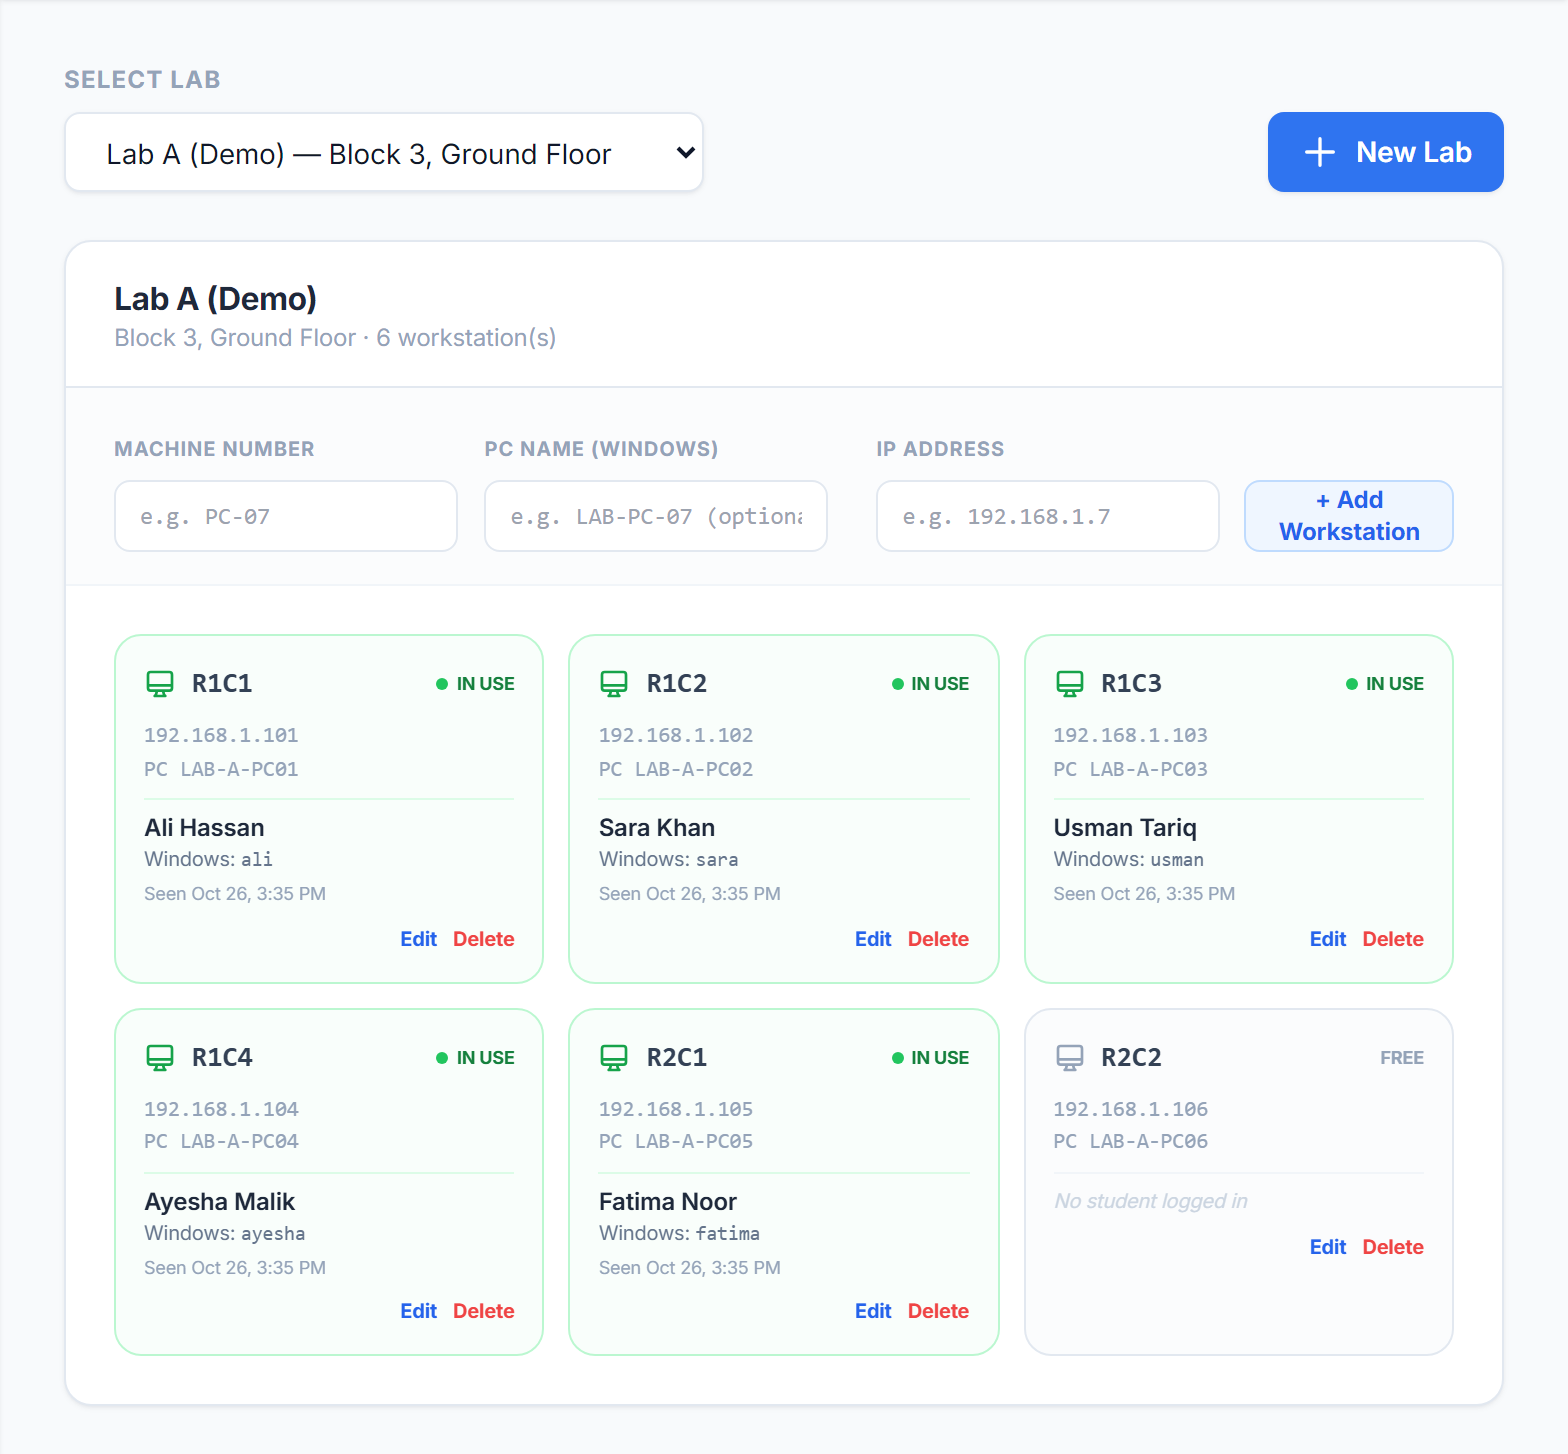
\includegraphics[width=\linewidth,height=418pt,keepaspectratio]{Figures/ui_labs_workstations.png}
\caption{Labs and Workstations}
\label{fig:ui_labs_workstations}
\end{figure}
\SoftBarrierN

The device-binding page (Figure~\ref{fig:ui_device_bindings}) lists each student's binding status, bound PC and last-seen time (FR1). \emph{Reset Binding} (\texttt{DELETE /api/users/\{id\}/device-binding}) removes the binding and revokes all the student's tokens, so the next login binds a new PC; \emph{Force Logout} only revokes the tokens. In the figure the five students who have signed in are \emph{Bound} to LAB-A-PC01 to LAB-A-PC05, while Hamza Iqbal is \emph{Unbound}, so his row has no PC and no actions. A search box and a \emph{Show unbound only} switch help the administrator find a student, and the note at the top says that an administrator can reset a binding after a genuine hardware change or a login problem.

\begin{figure}[tbp]
\centering
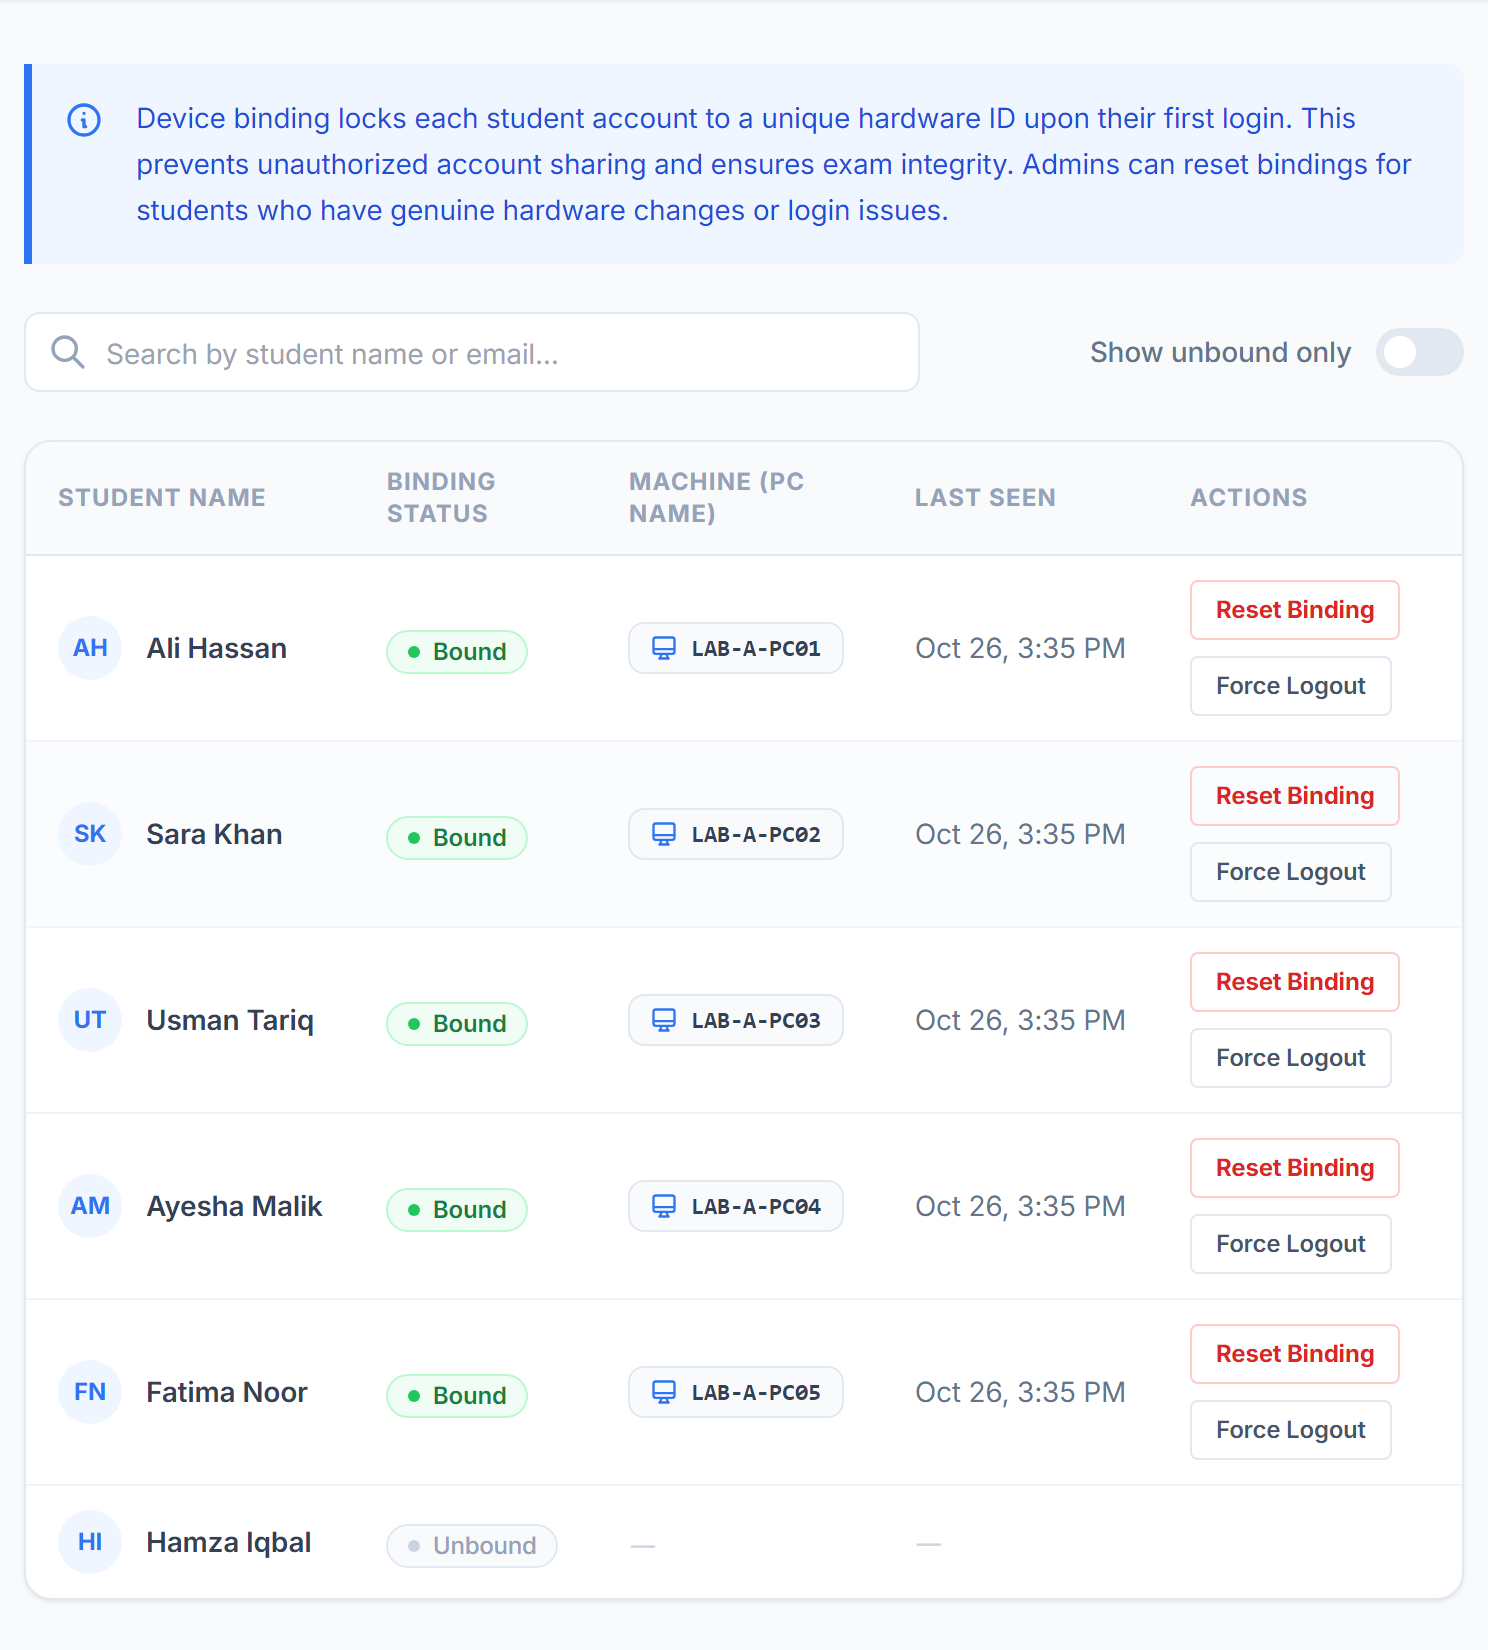
\includegraphics[width=\linewidth,height=500pt,keepaspectratio]{Figures/ui_device_bindings.png}
\caption{Device Bindings (Email, Windows User and Registered Columns Omitted)}
\label{fig:ui_device_bindings}
\end{figure}
\SoftBarrierN

The read-only audit page (Figure~\ref{fig:ui_audit_logs}) lists \texttt{AuditLogs} rows (time, actor, event, entity, JSON details) for security-relevant and staff actions, such as logins, grade overrides, completed AI grading and submissions (FR12). The newest rows come first, and the actor is a user with an email or \emph{System} for background jobs. The visible rows follow the end of the demo exam, from the warning sent to Usman (\texttt{PROCTOR\_WARNING\_SENT}, 3:35:43~PM) through three submissions (\texttt{SESSION\_SUBMITTED}) and the background grading (\texttt{AI\_GRADING\_COMPLETED}) to a grade override by Dr. Ahmed and a new login by Ali Hassan. The green badge \emph{Chain verified (91 entries)} at the top shows that the hash chain over these rows verifies, and \emph{Re-verify} runs the check again.

\begin{figure}[tbp]
\centering
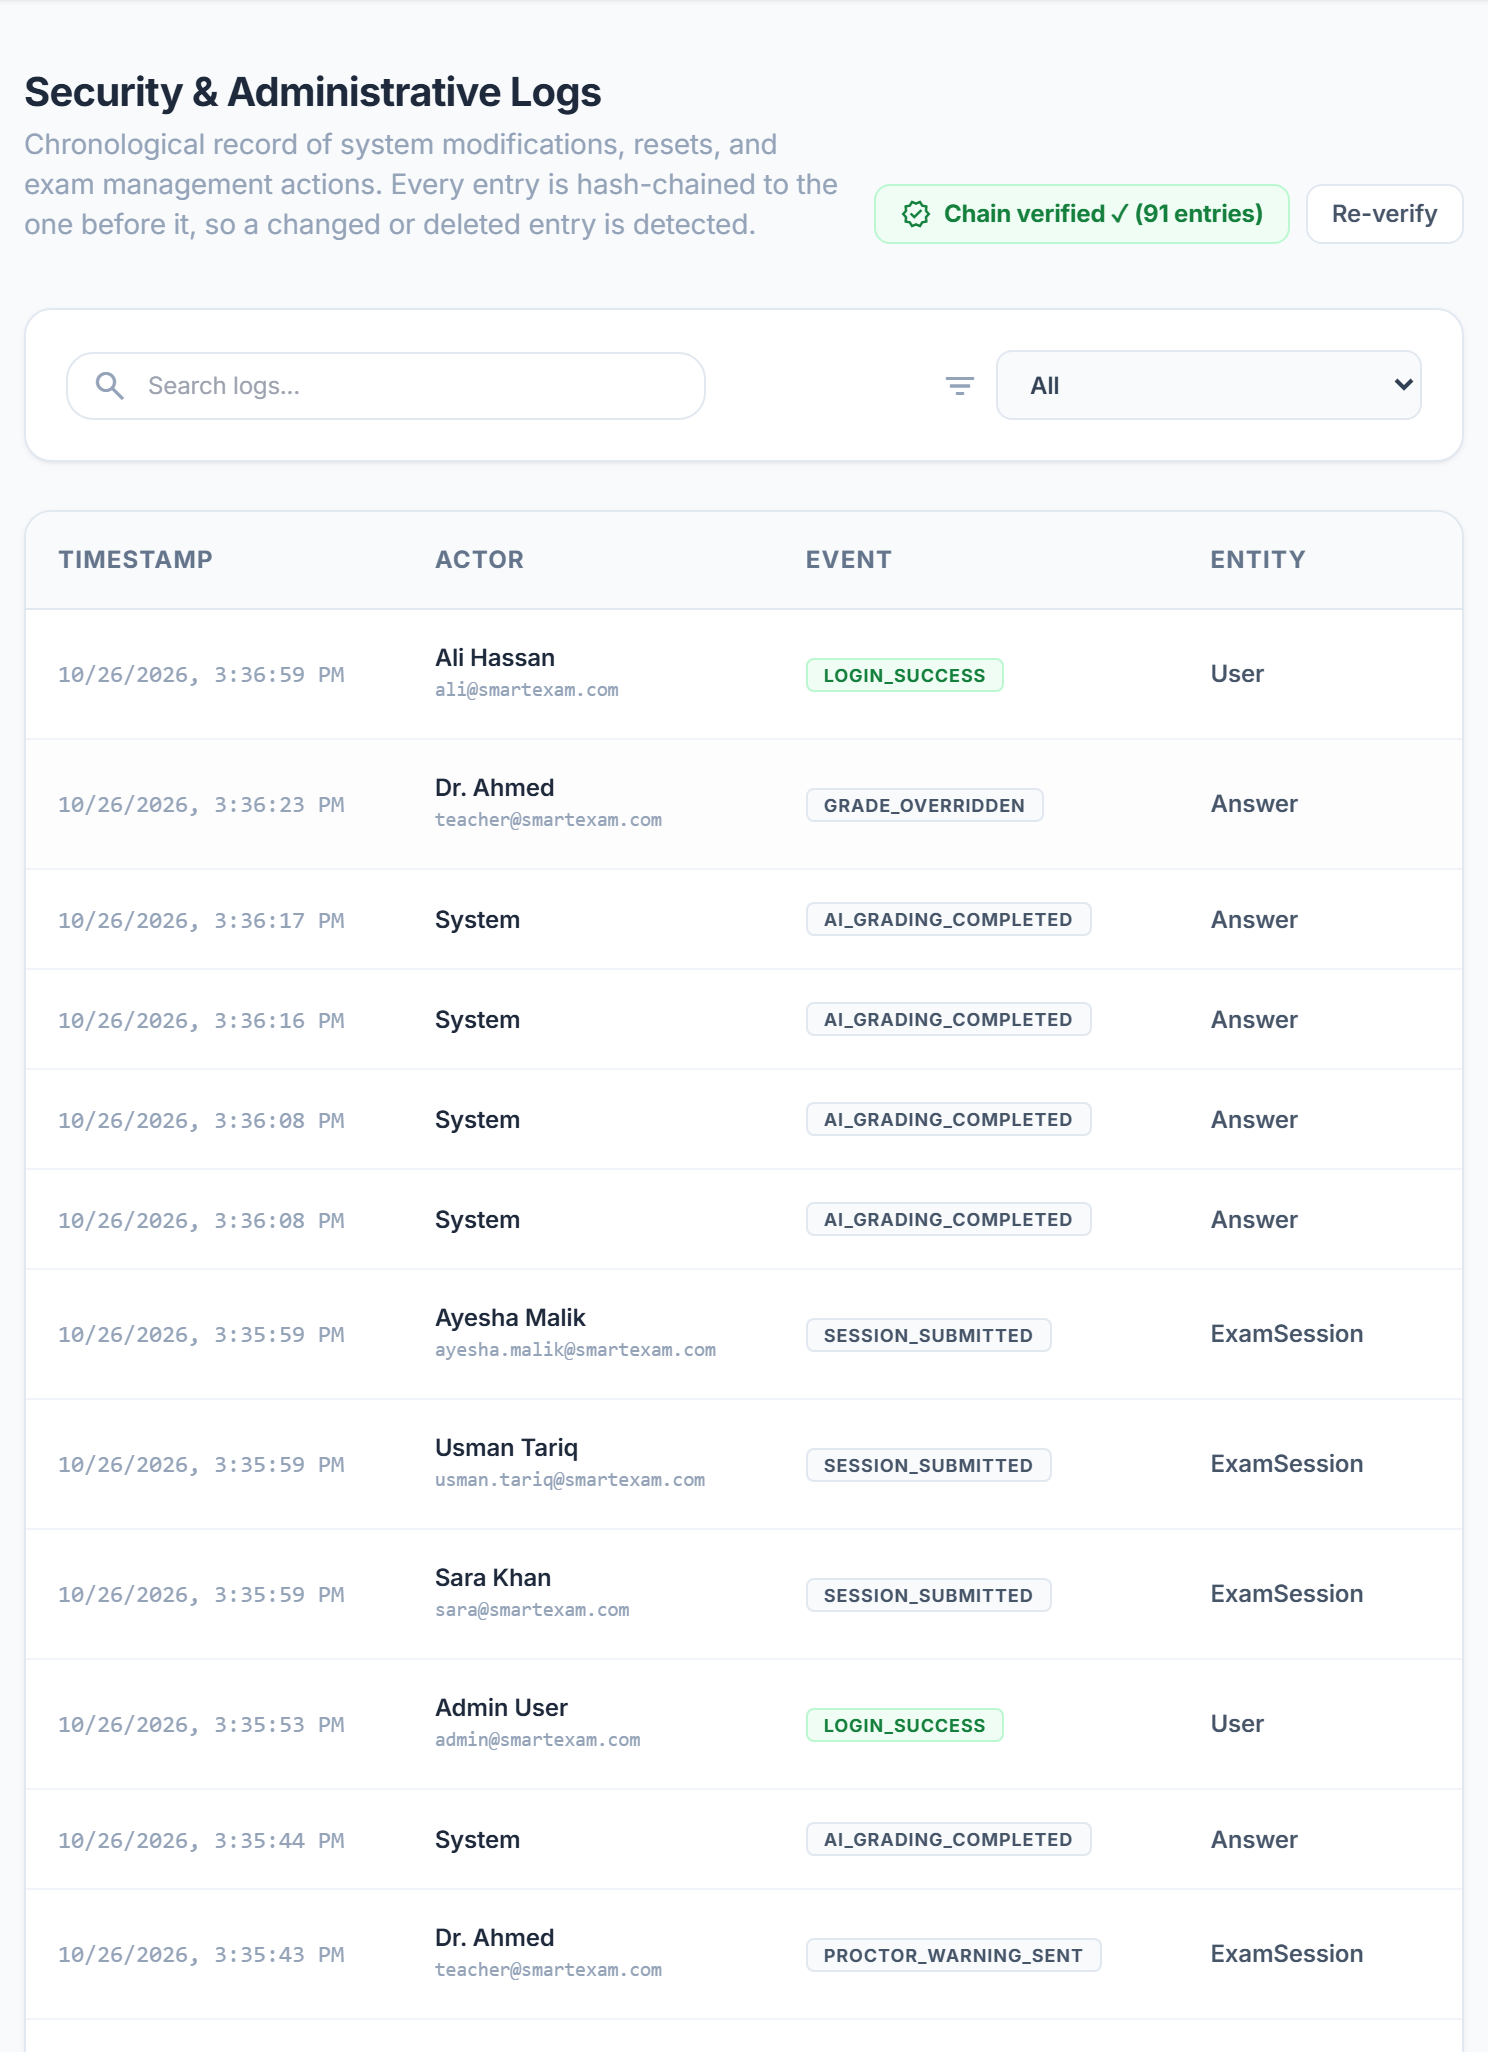
\includegraphics[width=\linewidth,height=622pt,keepaspectratio]{Figures/ui_audit_logs.png}
\caption{Audit Log Page (Details Column Omitted)}
\label{fig:ui_audit_logs}
\end{figure}
\SoftBarrierN

In the student portal (Figures~\ref{fig:ui_student_performance} to~\ref{fig:ui_student_performance_b}) a student sees exams taken, average and best score, integrity flags, a score trend, the score of each exam and an exam timeline; practice exams do not count towards results (they are auto-marked but never plagiarism-checked and are hidden from the student's results). The summary cards (Figure~\ref{fig:ui_student_performance}) show four exams taken, an average of 85.9\,\%, a best score of 93.3\,\% and no flags; the flag count adds up the violations recorded in the student's sessions. The average matches the mean of the four scores in the timeline (80, 83.3, 93.3 and 87.1\,\%).

\begin{figure}[tbp]
\centering
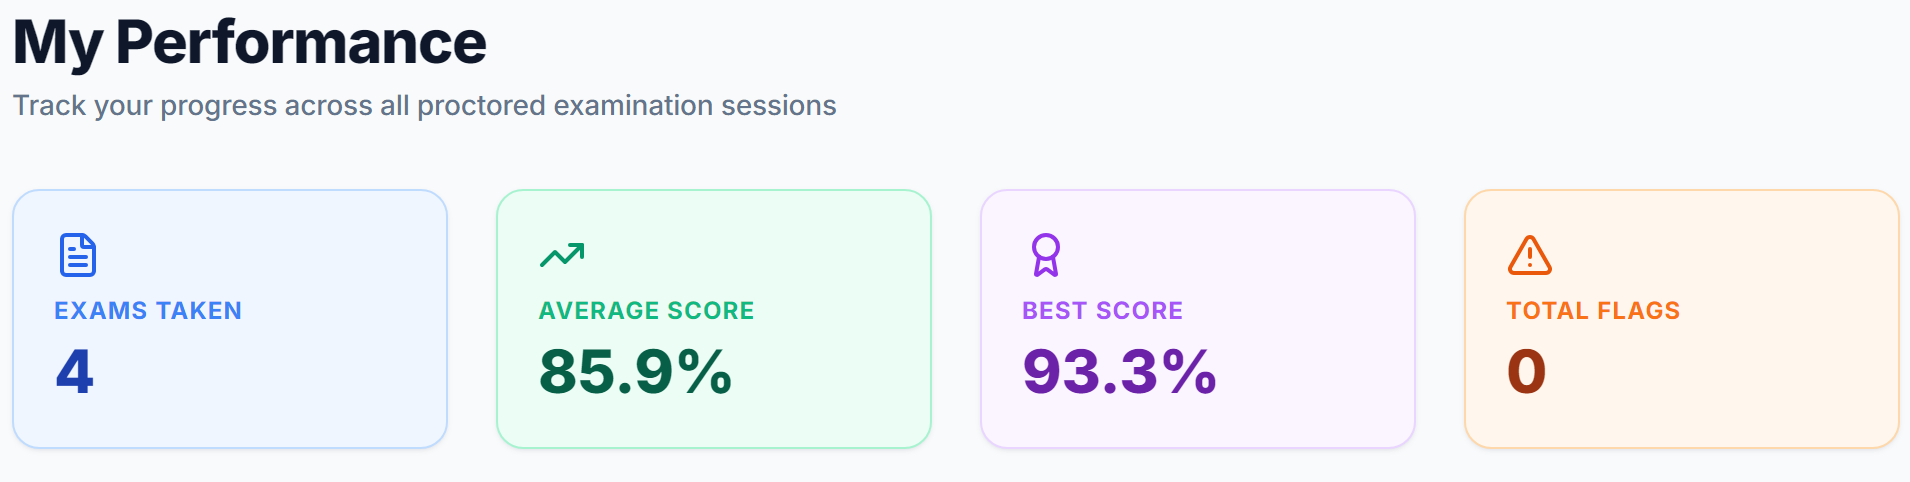
\includegraphics[width=\linewidth]{Figures/ui_student_performance_a_p1.png}
\caption{Student Performance Page (a): Summary Cards}
\label{fig:ui_student_performance}
\end{figure}
\SoftBarrierN

The \emph{Score Over Time} chart (Figure~\ref{fig:ui_student_performance_trend}) draws the same scores in date order, from Lab Exam~1 to the Mid-Term Lab Exam, above a dashed pass-mark line at 50\,\%. The \emph{Improving trend} badge appears because the latest score is higher than the first one. Figure~\ref{fig:ui_student_performance_b} shows the four exams again as bars, with the score rounded to a whole percent, and as a timeline, newest first, with the date and exact score of each exam.

\begin{figure}[tbp]
\centering
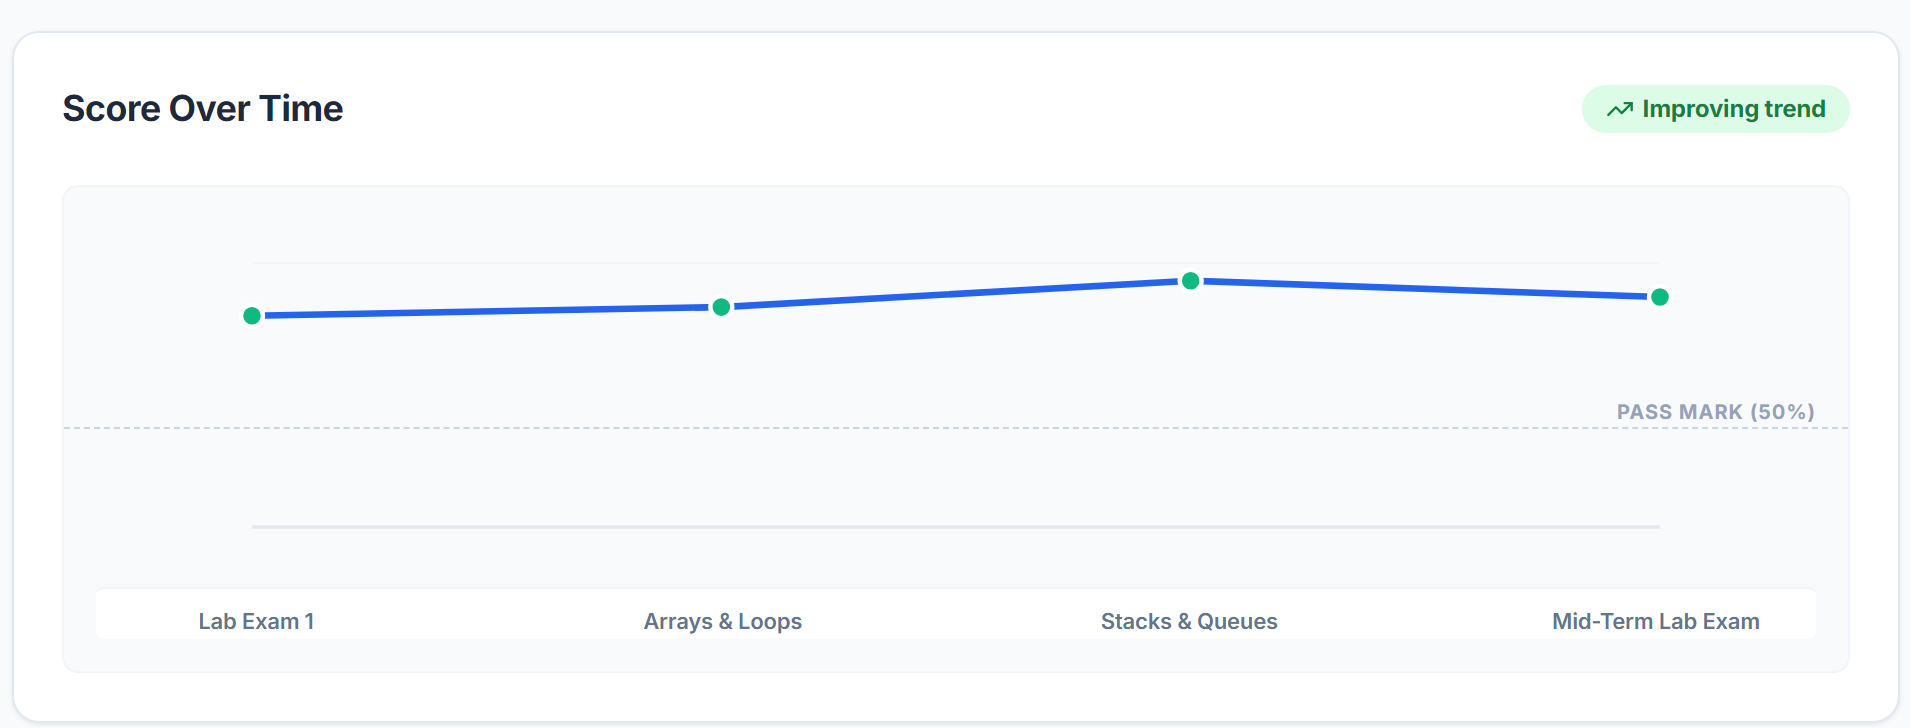
\includegraphics[width=\linewidth]{Figures/ui_student_performance_a_p2.png}
\caption{Student Performance Page (b): Score Trend}
\label{fig:ui_student_performance_trend}
\end{figure}
\SoftBarrierN

\begin{figure}[tbp]
\centering
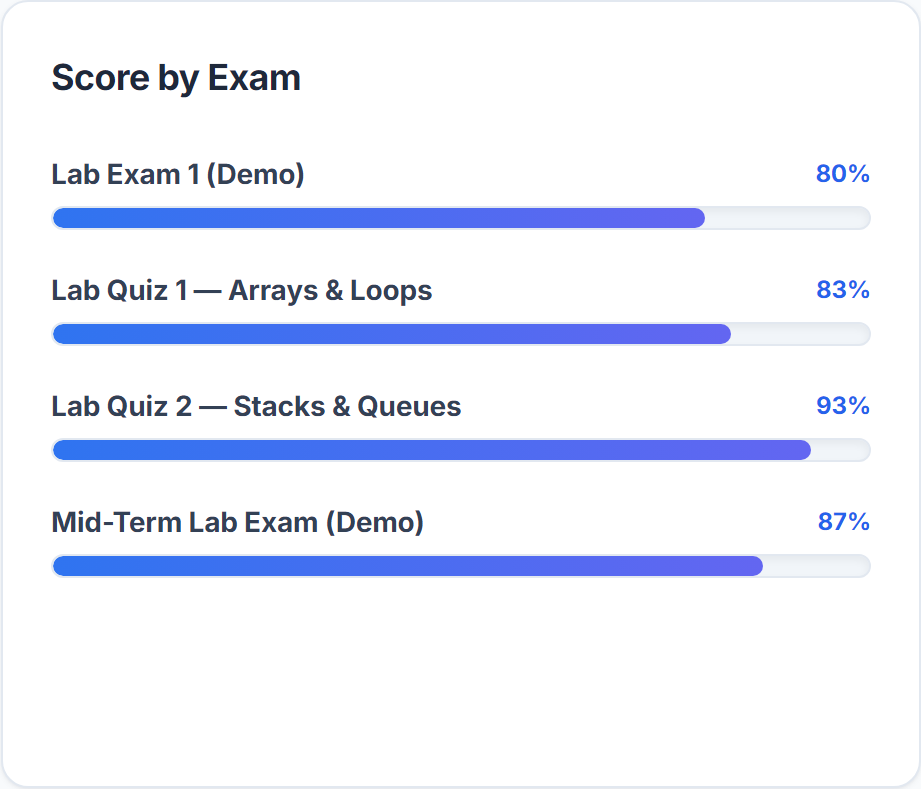
\includegraphics[width=0.7\linewidth]{Figures/ui_student_performance_scores.png}\\[4pt]
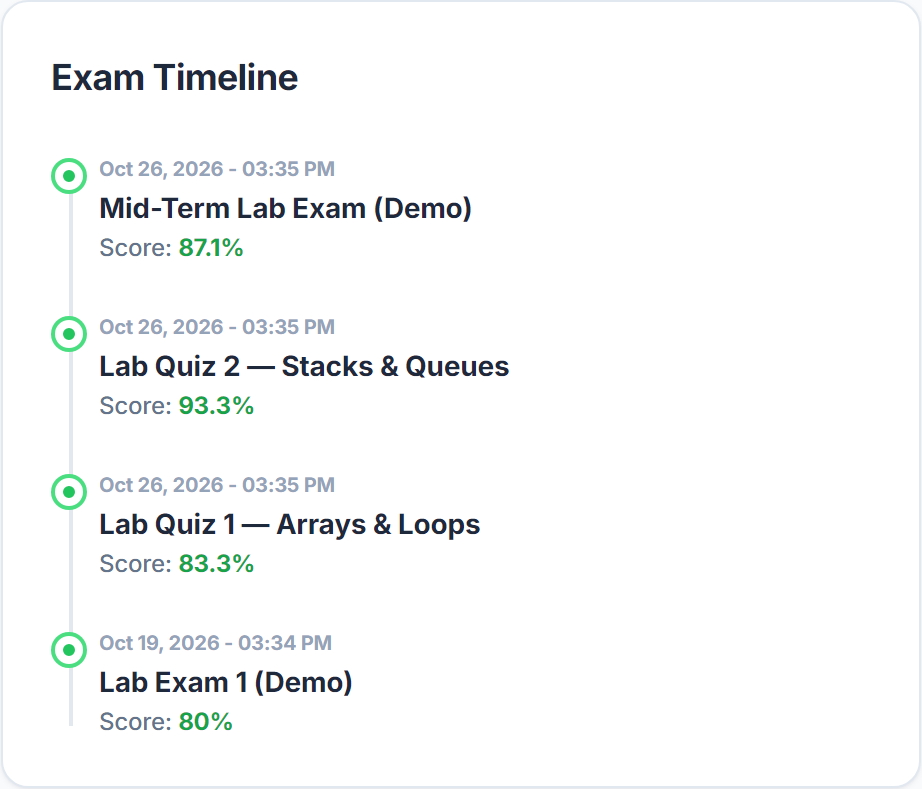
\includegraphics[width=0.7\linewidth]{Figures/ui_student_performance_timeline.png}
\caption{Student Performance Page (c): Score by Exam and Exam Timeline Cards}
\label{fig:ui_student_performance_b}
\end{figure}
\SoftBarrierN

\clearpage
\renewcommand{\topfraction}{0.7}\renewcommand{\bottomfraction}{0.3}
\renewcommand{\textfraction}{0.2}\renewcommand{\floatpagefraction}{0.5}
\section{Physical Database Tables}
\label{sec:physical_tables}
% Database tables, one per entity of the ERD (Figures erd_diagram and erd_diagram_b), in ERD order.
% Columns, types, keys and lengths follow Backend_API/Data/AppDbContext.cs and the EF Core model snapshot.

\label{sec:db_tables_detail}
This section gives one table for each entity of the ERD (Figures~\ref{fig:erd_diagram} and~\ref{fig:erd_diagram_b}), in the same order as the diagram, 29 tables in all. Each table lists every column that EF Core creates in PostgreSQL, with its data type, its key or constraint and a short description. In the tables, PK means primary key, FK means foreign key (the table it points to is in brackets), \texttt{uuid} is a globally unique identifier and \texttt{timestamptz} is a timestamp with time zone; key columns are never null, and a column marked ``no FK'' holds an id without a foreign-key constraint.

\par\ifdim\dimexpr\pagegoal-\pagetotal\relax<362pt\newpage\fi
\subsection{Users Table}
The \texttt{Users} table stores every account in the system, for all five roles: SuperAdmin, Admin, Teacher, Invigilator and Student. Most other tables point to it, for example \texttt{DeviceBindings}, \texttt{Sections} for the teacher and \texttt{ExamSessions} for the student. \texttt{Email} is unique, and \texttt{RollNumber} is unique whenever it is set.

{\small
\begin{longtable}{>{\raggedright\arraybackslash}p{3.4cm}>{\raggedright\arraybackslash}p{2.6cm}>{\raggedright\arraybackslash}p{2.6cm}>{\raggedright\arraybackslash}p{5.6cm}}
\caption{Users Table}\label{tab:db_users}\\
\hline\hline
\textbf{Field Name} & \textbf{Data Type} & \textbf{Key / Constraint} & \textbf{Description} \\ \hline
\endfirsthead
\multicolumn{4}{c}{\tablename~\thetable{} -- continued from previous page}\\
\hline\hline
\textbf{Field Name} & \textbf{Data Type} & \textbf{Key / Constraint} & \textbf{Description} \\ \hline
\endhead
\hline \multicolumn{4}{r}{Continued on next page}\\
\endfoot
\hline\hline
\endlastfoot
UserId & uuid & PK & Unique id of the user \\*
Name & text & Not null & Display name \\*
Email & text & Not null, unique & Email address, used to log in \\
RollNumber & varchar(32) & Null, unique when set & University roll number, stored in upper case; students may log in with it \\
PasswordHash & text & Not null & Salted PBKDF2 hash of the password \\
Salt & text & Not null & Random salt used for the hash \\*
Role & text & Not null & SuperAdmin, Admin, Teacher, Invigilator or Student \\*
IsActive & boolean & Not null & False when the account is deactivated; default true \\*
CreatedAt & timestamptz & Not null & When the account was created \\
\end{longtable}
}

\par\ifdim\dimexpr\pagegoal-\pagetotal\relax<362pt\newpage\fi
\subsection{DeviceBindings Table}
The \texttt{DeviceBindings} table links a user to the one PC the account is bound to. \texttt{UserId} is a foreign key to \texttt{Users} and is also unique, so a user has at most one binding, and the binding is deleted together with the user.

{\small
\begin{longtable}{>{\raggedright\arraybackslash}p{3.4cm}>{\raggedright\arraybackslash}p{2.6cm}>{\raggedright\arraybackslash}p{2.6cm}>{\raggedright\arraybackslash}p{5.6cm}}
\caption{DeviceBindings Table}\label{tab:db_devicebindings}\\
\hline\hline
\textbf{Field Name} & \textbf{Data Type} & \textbf{Key / Constraint} & \textbf{Description} \\ \hline
\endfirsthead
\multicolumn{4}{c}{\tablename~\thetable{} -- continued from previous page}\\
\hline\hline
\textbf{Field Name} & \textbf{Data Type} & \textbf{Key / Constraint} & \textbf{Description} \\ \hline
\endhead
\hline \multicolumn{4}{r}{Continued on next page}\\
\endfoot
\hline\hline
\endlastfoot
BindingId & uuid & PK & Unique id of the binding \\*
UserId & uuid & FK (Users), unique & The bound user \\*
HwidHash & text & Not null & SHA-256 hash of the PC's hardware fingerprint \\
HwidVersion & integer & Not null & Fingerprint format: 1 = old, 2 = current; default 1 \\
MachineName & text & Null & Windows computer name, e.g. LAB-PC-07 \\*
WindowsUsername & text & Null & Windows account logged in on that PC \\*
RegisteredAt & timestamptz & Not null & When the PC was bound \\*
LastSeenAt & timestamptz & Not null & Last time the bound PC was seen \\
\end{longtable}
}

\par\ifdim\dimexpr\pagegoal-\pagetotal\relax<314pt\newpage\fi
\subsection{UserSessions Table}
The \texttt{UserSessions} table keeps one row for each access token issued at login, stored by its JWT ID, so that a token can be revoked before it expires. A user can have many rows, and the rows are deleted with the user. \texttt{Jti} is unique.

{\small
\begin{longtable}{>{\raggedright\arraybackslash}p{3.4cm}>{\raggedright\arraybackslash}p{2.6cm}>{\raggedright\arraybackslash}p{2.6cm}>{\raggedright\arraybackslash}p{5.6cm}}
\caption{UserSessions Table}\label{tab:db_usersessions}\\
\hline\hline
\textbf{Field Name} & \textbf{Data Type} & \textbf{Key / Constraint} & \textbf{Description} \\ \hline
\endfirsthead
\multicolumn{4}{c}{\tablename~\thetable{} -- continued from previous page}\\
\hline\hline
\textbf{Field Name} & \textbf{Data Type} & \textbf{Key / Constraint} & \textbf{Description} \\ \hline
\endhead
\hline \multicolumn{4}{r}{Continued on next page}\\
\endfoot
\hline\hline
\endlastfoot
SessionId & uuid & PK & Unique id of the row \\*
UserId & uuid & FK (Users) & Owner of the token \\*
Jti & text & Not null, unique & JWT ID of the access token \\*
ExpiresAt & timestamptz & Not null & When the token expires \\*
IsRevoked & boolean & Not null & True once the token is revoked; default false \\*
CreatedAt & timestamptz & Not null & When the token was issued \\
\end{longtable}
}

\par\ifdim\dimexpr\pagegoal-\pagetotal\relax<362pt\newpage\fi
\subsection{RefreshTokens Table}
The \texttt{RefreshTokens} table stores the rotating refresh tokens; only the SHA-256 hash of each token is kept, never the token itself. Every login starts a new token family, and each refresh revokes the used token and issues the next one in the same family. Each row belongs to one user and is deleted with that user; \texttt{TokenHash} is unique.

{\small
\begin{longtable}{>{\raggedright\arraybackslash}p{3.4cm}>{\raggedright\arraybackslash}p{2.6cm}>{\raggedright\arraybackslash}p{2.6cm}>{\raggedright\arraybackslash}p{5.6cm}}
\caption{RefreshTokens Table}\label{tab:db_refreshtokens}\\
\hline\hline
\textbf{Field Name} & \textbf{Data Type} & \textbf{Key / Constraint} & \textbf{Description} \\ \hline
\endfirsthead
\multicolumn{4}{c}{\tablename~\thetable{} -- continued from previous page}\\
\hline\hline
\textbf{Field Name} & \textbf{Data Type} & \textbf{Key / Constraint} & \textbf{Description} \\ \hline
\endhead
\hline \multicolumn{4}{r}{Continued on next page}\\
\endfoot
\hline\hline
\endlastfoot
TokenId & uuid & PK & Unique id of the token \\*
UserId & uuid & FK (Users) & Owner of the token \\*
FamilyId & uuid & Not null, indexed & Token family started at login \\
TokenHash & varchar(64) & Not null, unique & SHA-256 hash of the raw token \\
Jti & varchar(64) & Not null, indexed & JWT ID of the access token issued with it \\
Channel & varchar(32) & Not null & web or student-client \\
MachineName & varchar(128) & Null & PC name, sent again as the machine claim on refresh \\
CreatedAt & timestamptz & Not null & When the token was issued \\
ExpiresAt & timestamptz & Not null & Fixed expiry; rotation does not extend it \\
RevokedAt & timestamptz & Null, concurrency token & When the token was revoked \\*
RevokedReason & varchar(32) & Null & Why it was revoked, e.g. rotated, reuse or logout \\*
Replaced\allowbreak By\allowbreak Token\allowbreak Id & uuid & Null, no~FK & Token that replaced it on rotation \\*
CreatedByIp & varchar(64) & Null & IP address the token was issued to \\
\end{longtable}
}

\par\ifdim\dimexpr\pagegoal-\pagetotal\relax<362pt\newpage\fi
\subsection{Notifications Table}
The \texttt{Notifications} table stores the in-app notifications, such as a new exam or released grades. Each row has one recipient in \texttt{Users} and is deleted with that user. An index on (\texttt{RecipientId}, \texttt{IsRead}) makes the unread list fast to read.

{\small
\begin{longtable}{>{\raggedright\arraybackslash}p{3.4cm}>{\raggedright\arraybackslash}p{2.6cm}>{\raggedright\arraybackslash}p{2.6cm}>{\raggedright\arraybackslash}p{5.6cm}}
\caption{Notifications Table}\label{tab:db_notifications}\\
\hline\hline
\textbf{Field Name} & \textbf{Data Type} & \textbf{Key / Constraint} & \textbf{Description} \\ \hline
\endfirsthead
\multicolumn{4}{c}{\tablename~\thetable{} -- continued from previous page}\\
\hline\hline
\textbf{Field Name} & \textbf{Data Type} & \textbf{Key / Constraint} & \textbf{Description} \\ \hline
\endhead
\hline \multicolumn{4}{r}{Continued on next page}\\
\endfoot
\hline\hline
\endlastfoot
NotificationId & uuid & PK & Unique id of the notification \\*
RecipientId & uuid & FK (Users) & User who receives it \\*
Title & text & Not null & Short title \\
Body & text & Not null & Message text \\
Type & text & Not null & Kind, e.g. ExamScheduled or GradeReleased \\
IsRead & boolean & Not null & True once the user has read it \\*
EmailSent & boolean & Not null & True if it was also sent by email \\*
RelatedEntityId & text & Null & Id of the exam or session it is about \\*
CreatedAt & timestamptz & Not null & When it was created \\
\end{longtable}
}

\par\ifdim\dimexpr\pagegoal-\pagetotal\relax<218pt\newpage\fi
\subsection{Departments Table}
The \texttt{Departments} table stores the academic departments. Each department has many courses in \texttt{Courses}, and a department that still has courses cannot be deleted. The department name is unique.

{\small
\begin{longtable}{>{\raggedright\arraybackslash}p{3.4cm}>{\raggedright\arraybackslash}p{2.6cm}>{\raggedright\arraybackslash}p{2.6cm}>{\raggedright\arraybackslash}p{5.6cm}}
\caption{Departments Table}\label{tab:db_departments}\\
\hline\hline
\textbf{Field Name} & \textbf{Data Type} & \textbf{Key / Constraint} & \textbf{Description} \\ \hline
\endfirsthead
\multicolumn{4}{c}{\tablename~\thetable{} -- continued from previous page}\\
\hline\hline
\textbf{Field Name} & \textbf{Data Type} & \textbf{Key / Constraint} & \textbf{Description} \\ \hline
\endhead
\hline \multicolumn{4}{r}{Continued on next page}\\
\endfoot
\hline\hline
\endlastfoot
DeptId & uuid & PK & Unique id of the department \\*
Name & text & Not null, unique & Department name \\*
\end{longtable}
}

\par\ifdim\dimexpr\pagegoal-\pagetotal\relax<266pt\newpage\fi
\subsection{Courses Table}
The \texttt{Courses} table stores the courses offered by each department. Every course belongs to one department through \texttt{DeptId}, and the course code is unique within its department. A course has many sections in \texttt{Sections}.

{\small
\begin{longtable}{>{\raggedright\arraybackslash}p{3.4cm}>{\raggedright\arraybackslash}p{2.6cm}>{\raggedright\arraybackslash}p{2.6cm}>{\raggedright\arraybackslash}p{5.6cm}}
\caption{Courses Table}\label{tab:db_courses}\\
\hline\hline
\textbf{Field Name} & \textbf{Data Type} & \textbf{Key / Constraint} & \textbf{Description} \\ \hline
\endfirsthead
\multicolumn{4}{c}{\tablename~\thetable{} -- continued from previous page}\\
\hline\hline
\textbf{Field Name} & \textbf{Data Type} & \textbf{Key / Constraint} & \textbf{Description} \\ \hline
\endhead
\hline \multicolumn{4}{r}{Continued on next page}\\
\endfoot
\hline\hline
\endlastfoot
CourseId & uuid & PK & Unique id of the course \\*
DeptId & uuid & FK (Departments) & Department that offers the course \\*
Name & text & Not null & Course name \\*
Code & text & Not null, unique with DeptId & Course code, e.g. CS301 \\
\end{longtable}
}

\par\ifdim\dimexpr\pagegoal-\pagetotal\relax<290pt\newpage\fi
\subsection{Sections Table}
The \texttt{Sections} table stores a class of a course in one semester, taught by one teacher. \texttt{CourseId} links it to \texttt{Courses}, and \texttt{TeacherId} links it to the teacher in \texttt{Users}; a teacher who still teaches a section cannot be deleted. Students join a section through \texttt{Section}\allowbreak\texttt{Enrollments}, and exams are created for a section.

{\small
\begin{longtable}{>{\raggedright\arraybackslash}p{3.4cm}>{\raggedright\arraybackslash}p{2.6cm}>{\raggedright\arraybackslash}p{2.6cm}>{\raggedright\arraybackslash}p{5.6cm}}
\caption{Sections Table}\label{tab:db_sections}\\
\hline\hline
\textbf{Field Name} & \textbf{Data Type} & \textbf{Key / Constraint} & \textbf{Description} \\ \hline
\endfirsthead
\multicolumn{4}{c}{\tablename~\thetable{} -- continued from previous page}\\
\hline\hline
\textbf{Field Name} & \textbf{Data Type} & \textbf{Key / Constraint} & \textbf{Description} \\ \hline
\endhead
\hline \multicolumn{4}{r}{Continued on next page}\\
\endfoot
\hline\hline
\endlastfoot
SectionId & uuid & PK & Unique id of the section \\*
CourseId & uuid & FK (Courses) & Course of the section \\*
TeacherId & uuid & FK (Users) & Teacher of the section \\*
Name & text & Not null & Section name \\*
Semester & text & Not null & Semester of the section \\
\end{longtable}
}

\par\ifdim\dimexpr\pagegoal-\pagetotal\relax<242pt\newpage\fi
\subsection{SectionEnrollments Table}
The \texttt{SectionEnrollments} table records which students are enrolled in which section. Each row joins one section to one student in \texttt{Users}, and it is deleted when either of them is deleted.

{\small
\begin{longtable}{>{\raggedright\arraybackslash}p{3.4cm}>{\raggedright\arraybackslash}p{2.6cm}>{\raggedright\arraybackslash}p{2.6cm}>{\raggedright\arraybackslash}p{5.6cm}}
\caption{SectionEnrollments Table}\label{tab:db_sectionenrollments}\\
\hline\hline
\textbf{Field Name} & \textbf{Data Type} & \textbf{Key / Constraint} & \textbf{Description} \\ \hline
\endfirsthead
\multicolumn{4}{c}{\tablename~\thetable{} -- continued from previous page}\\
\hline\hline
\textbf{Field Name} & \textbf{Data Type} & \textbf{Key / Constraint} & \textbf{Description} \\ \hline
\endhead
\hline \multicolumn{4}{r}{Continued on next page}\\
\endfoot
\hline\hline
\endlastfoot
EnrollmentId & uuid & PK & Unique id of the enrolment \\*
SectionId & uuid & FK (Sections) & The section \\*
UserId & uuid & FK (Users) & The enrolled student \\
\end{longtable}
}

\par\ifdim\dimexpr\pagegoal-\pagetotal\relax<338pt\newpage\fi
\subsection{AttendanceRecords Table}
The \texttt{AttendanceRecords} table stores a student's class attendance in one section, imported from the teacher's CSV file. There is one row per section and student, so a new import updates the row in place. Exam eligibility is recalculated from these rows by comparing attended with total classes against the exam's minimum attendance.

{\small
\begin{longtable}{>{\raggedright\arraybackslash}p{3.4cm}>{\raggedright\arraybackslash}p{2.6cm}>{\raggedright\arraybackslash}p{2.6cm}>{\raggedright\arraybackslash}p{5.6cm}}
\caption{AttendanceRecords Table}\label{tab:db_attendancerecords}\\
\hline\hline
\textbf{Field Name} & \textbf{Data Type} & \textbf{Key / Constraint} & \textbf{Description} \\ \hline
\endfirsthead
\multicolumn{4}{c}{\tablename~\thetable{} -- continued from previous page}\\
\hline\hline
\textbf{Field Name} & \textbf{Data Type} & \textbf{Key / Constraint} & \textbf{Description} \\ \hline
\endhead
\hline \multicolumn{4}{r}{Continued on next page}\\
\endfoot
\hline\hline
\endlastfoot
AttendanceId & uuid & PK & Unique id of the record \\*
SectionId & uuid & FK (Sections), unique with UserId & The section \\*
UserId & uuid & FK (Users) & The student \\
TotalClasses & integer & Not null & Number of classes held \\*
AttendedClasses & integer & Not null & Number of classes the student attended \\*
UpdatedAt & timestamptz & Not null & When the row was last imported \\*
ImportedBy & uuid & Null, no~FK & User who imported the file \\
\end{longtable}
}

\par\ifdim\dimexpr\pagegoal-\pagetotal\relax<266pt\newpage\fi
\subsection{Labs Table}
The \texttt{Labs} table stores the computer labs where exams are held. Each lab has many PCs in \texttt{Workstations}, which are deleted with the lab.

{\small
\begin{longtable}{>{\raggedright\arraybackslash}p{3.4cm}>{\raggedright\arraybackslash}p{2.6cm}>{\raggedright\arraybackslash}p{2.6cm}>{\raggedright\arraybackslash}p{5.6cm}}
\caption{Labs Table}\label{tab:db_labs}\\
\hline\hline
\textbf{Field Name} & \textbf{Data Type} & \textbf{Key / Constraint} & \textbf{Description} \\ \hline
\endfirsthead
\multicolumn{4}{c}{\tablename~\thetable{} -- continued from previous page}\\
\hline\hline
\textbf{Field Name} & \textbf{Data Type} & \textbf{Key / Constraint} & \textbf{Description} \\ \hline
\endhead
\hline \multicolumn{4}{r}{Continued on next page}\\
\endfoot
\hline\hline
\endlastfoot
LabId & uuid & PK & Unique id of the lab \\*
Name & text & Not null & Lab name \\*
Location & text & Not null & Where the lab is \\*
CreatedAt & timestamptz & Not null & When the lab was added \\
\end{longtable}
}

\par\ifdim\dimexpr\pagegoal-\pagetotal\relax<290pt\newpage\fi
\subsection{Workstations Table}
The \texttt{Workstations} table stores the lab PCs that are used as exam seats. Each PC belongs to one lab through \texttt{LabId}. A seat check compares the student client's computer name with \texttt{HostName}, or with \texttt{MachineNumber} when no host name is set.

{\small
\begin{longtable}{>{\raggedright\arraybackslash}p{3.4cm}>{\raggedright\arraybackslash}p{2.6cm}>{\raggedright\arraybackslash}p{2.6cm}>{\raggedright\arraybackslash}p{5.6cm}}
\caption{Workstations Table}\label{tab:db_workstations}\\
\hline\hline
\textbf{Field Name} & \textbf{Data Type} & \textbf{Key / Constraint} & \textbf{Description} \\ \hline
\endfirsthead
\multicolumn{4}{c}{\tablename~\thetable{} -- continued from previous page}\\
\hline\hline
\textbf{Field Name} & \textbf{Data Type} & \textbf{Key / Constraint} & \textbf{Description} \\ \hline
\endhead
\hline \multicolumn{4}{r}{Continued on next page}\\
\endfoot
\hline\hline
\endlastfoot
WorkstationId & uuid & PK & Unique id of the PC \\*
LabId & uuid & FK (Labs) & Lab the PC is in \\*
MachineNumber & text & Not null & Machine number of the seat \\*
IpAddress & text & Not null & IP address of the PC \\*
HostName & varchar(128) & Null & Windows computer name, e.g. LAB-PC-07 \\
\end{longtable}
}

\par\ifdim\dimexpr\pagegoal-\pagetotal\relax<362pt\newpage\fi
\subsection{Exams Table}
The \texttt{Exams} table stores each exam with its schedule and the rules the student client enforces. Every exam belongs to one section through \texttt{SectionId}. An exam has questions, assignments, sessions, proctors and reports in other tables, which point to it through \texttt{ExamId}.

{\small
\begin{longtable}{>{\raggedright\arraybackslash}p{3.4cm}>{\raggedright\arraybackslash}p{2.6cm}>{\raggedright\arraybackslash}p{2.6cm}>{\raggedright\arraybackslash}p{5.6cm}}
\caption{Exams Table}\label{tab:db_exams}\\
\hline\hline
\textbf{Field Name} & \textbf{Data Type} & \textbf{Key / Constraint} & \textbf{Description} \\ \hline
\endfirsthead
\multicolumn{4}{c}{\tablename~\thetable{} -- continued from previous page}\\
\hline\hline
\textbf{Field Name} & \textbf{Data Type} & \textbf{Key / Constraint} & \textbf{Description} \\ \hline
\endhead
\hline \multicolumn{4}{r}{Continued on next page}\\
\endfoot
\hline\hline
\endlastfoot
ExamId & uuid & PK & Unique id of the exam \\*
SectionId & uuid & FK (Sections) & Section the exam is for \\*
Title & text & Not null & Exam title \\
Instructions & text & Null & Shown on the student exam dashboard \\
StartTime & timestamptz & Not null & Scheduled start \\
DurationMinutes & integer & Not null & Length of the exam in minutes \\
Early\allowbreak Join\allowbreak Minutes & integer & Not null & Minutes before the start that students may begin; 0 = at the start \\
AllowedApps & text & Not null & JSON list of allowed programs, e.g. code.exe \\
Ai\allowbreak Evaluation\allowbreak Enabled & boolean & Not null & Turns automatic grading on; default true \\
Plagiarism\allowbreak Threshold & integer & Not null & Similarity percent at which a pair is flagged; default 70 \\
LockdownMode & varchar(16) & Not null & Off, Report or Enforce; default Report \\
Block\allowbreak Multi\allowbreak Monitor & boolean & Not null & Block a second monitor; default true \\
Require\allowbreak Readiness & boolean & Not null & Start needs a passing readiness check at most 30 minutes old \\
RequireWebcam & boolean & Not null & Exam needs a webcam \\
RequireMic & boolean & Not null & Exam needs a microphone \\
IsMock & boolean & Not null & Practice exam: unlimited attempts, left out of results and plagiarism \\
Min\allowbreak Attendance\allowbreak Percent & double precision & Not null & Attendance needed to be eligible; default 75 \\
EnforceSeat & boolean & Not null & Student may only sit at the assigned seat; default true \\
Screenshot\allowbreak Interval\allowbreak Seconds & integer & Not null & Mean time between screenshots; default 60 \\*
Webcam\allowbreak Interval\allowbreak Seconds & integer & Not null & Mean time between webcam snapshots; default 60 \\*
Status & text & Not null & Scheduled, Active or Ended; default Scheduled \\*
CreatedAt & timestamptz & Not null & When the exam was created \\
\end{longtable}
}

\par\ifdim\dimexpr\pagegoal-\pagetotal\relax<362pt\newpage\fi
\subsection{ExamAssignments Table}
The \texttt{ExamAssignments} table is the roster of an exam: it joins a student to an exam and holds the eligibility decision and the optional seat. \texttt{ExamId} and \texttt{UserId} are required foreign keys, while \texttt{WorkstationId} may be empty when no seat is assigned. A teacher's manual decision is marked so that a recalculation from attendance leaves it alone.

{\small
\begin{longtable}{>{\raggedright\arraybackslash}p{3.4cm}>{\raggedright\arraybackslash}p{2.6cm}>{\raggedright\arraybackslash}p{2.6cm}>{\raggedright\arraybackslash}p{5.6cm}}
\caption{ExamAssignments Table}\label{tab:db_examassignments}\\
\hline\hline
\textbf{Field Name} & \textbf{Data Type} & \textbf{Key / Constraint} & \textbf{Description} \\ \hline
\endfirsthead
\multicolumn{4}{c}{\tablename~\thetable{} -- continued from previous page}\\
\hline\hline
\textbf{Field Name} & \textbf{Data Type} & \textbf{Key / Constraint} & \textbf{Description} \\ \hline
\endhead
\hline \multicolumn{4}{r}{Continued on next page}\\
\endfoot
\hline\hline
\endlastfoot
AssignmentId & uuid & PK & Unique id of the assignment \\*
ExamId & uuid & FK (Exams) & The exam \\*
UserId & uuid & FK (Users) & The student \\
WorkstationId & uuid & FK (Workstations), null & Assigned seat, if any \\
IsEligible & boolean & Not null & Whether the student may sit the exam; default true \\*
EligibilityNote & text & Null & Reason for the eligibility decision \\*
Eligibility\allowbreak Overridden & boolean & Not null & True when a teacher decided by hand \\*
Eligibility\allowbreak Source & varchar(16) & Null & Attendance or Manual \\
\end{longtable}
}

\par\ifdim\dimexpr\pagegoal-\pagetotal\relax<266pt\newpage\fi
\subsection{ExamProctors Table}
The \texttt{ExamProctors} table records which staff members supervise which exam. It is the only table with a composite primary key, (\texttt{ExamId}, \texttt{UserId}), so a person is assigned to an exam at most once. \texttt{AssignedBy} is a plain id without a foreign key, so the row stays even if the assigning account is removed.

{\small
\begin{longtable}{>{\raggedright\arraybackslash}p{3.4cm}>{\raggedright\arraybackslash}p{2.6cm}>{\raggedright\arraybackslash}p{2.6cm}>{\raggedright\arraybackslash}p{5.6cm}}
\caption{ExamProctors Table}\label{tab:db_examproctors}\\
\hline\hline
\textbf{Field Name} & \textbf{Data Type} & \textbf{Key / Constraint} & \textbf{Description} \\ \hline
\endfirsthead
\multicolumn{4}{c}{\tablename~\thetable{} -- continued from previous page}\\
\hline\hline
\textbf{Field Name} & \textbf{Data Type} & \textbf{Key / Constraint} & \textbf{Description} \\ \hline
\endhead
\hline \multicolumn{4}{r}{Continued on next page}\\
\endfoot
\hline\hline
\endlastfoot
ExamId & uuid & PK, FK (Exams) & The exam \\*
UserId & uuid & PK, FK (Users) & Staff member who supervises it \\*
AssignedBy & uuid & Not null, no~FK & User who made the assignment \\*
AssignedAt & timestamptz & Not null & When the assignment was made \\
\end{longtable}
}

\par\ifdim\dimexpr\pagegoal-\pagetotal\relax<362pt\newpage\fi
\subsection{AuditLogs Table}
The \texttt{AuditLogs} table stores a record of security-relevant and staff actions. It has no foreign keys: the rows are linked into a hash chain by \texttt{Sequence}, \texttt{PrevHash} and \texttt{Hash}, so a changed or deleted row can be detected. \texttt{ActorId} is a plain indexed id, so it keeps the user's id even after that user is deleted.

{\small
\begin{longtable}{>{\raggedright\arraybackslash}p{3.4cm}>{\raggedright\arraybackslash}p{2.6cm}>{\raggedright\arraybackslash}p{2.6cm}>{\raggedright\arraybackslash}p{5.6cm}}
\caption{AuditLogs Table}\label{tab:db_auditlogs}\\
\hline\hline
\textbf{Field Name} & \textbf{Data Type} & \textbf{Key / Constraint} & \textbf{Description} \\ \hline
\endfirsthead
\multicolumn{4}{c}{\tablename~\thetable{} -- continued from previous page}\\
\hline\hline
\textbf{Field Name} & \textbf{Data Type} & \textbf{Key / Constraint} & \textbf{Description} \\ \hline
\endhead
\hline \multicolumn{4}{r}{Continued on next page}\\
\endfoot
\hline\hline
\endlastfoot
LogId & uuid & PK & Unique id of the record \\*
ActorId & uuid & Null, indexed, no~FK & User who acted; null for system events \\*
EventType & text & Not null & Action, e.g. LOGIN\_SUCCESS \\
EntityType & text & Not null & Kind of record acted on, e.g. User \\
EntityId & text & Null & Id of that record \\
Details & text & Not null & Details as JSON \\
CreatedAt & timestamptz & Not null & When the action happened \\*
Sequence & bigint & Null, unique & Position in the hash chain \\*
PrevHash & varchar(64) & Null & Hash of the previous row \\*
Hash & varchar(64) & Null & SHA-256 hash of this row \\
\end{longtable}
}

\par\ifdim\dimexpr\pagegoal-\pagetotal\relax<362pt\newpage\fi
\subsection{Questions Table}
The \texttt{Questions} table stores the questions of each exam, which may be coding, theory or multiple-choice questions. Every question belongs to one exam through \texttt{ExamId}. A coding question has test cases in \texttt{TestCases}, and the students' answers point to the question from \texttt{Answers}.

{\small
\begin{longtable}{>{\raggedright\arraybackslash}p{3.4cm}>{\raggedright\arraybackslash}p{2.6cm}>{\raggedright\arraybackslash}p{2.6cm}>{\raggedright\arraybackslash}p{5.6cm}}
\caption{Questions Table}\label{tab:db_questions}\\
\hline\hline
\textbf{Field Name} & \textbf{Data Type} & \textbf{Key / Constraint} & \textbf{Description} \\ \hline
\endfirsthead
\multicolumn{4}{c}{\tablename~\thetable{} -- continued from previous page}\\
\hline\hline
\textbf{Field Name} & \textbf{Data Type} & \textbf{Key / Constraint} & \textbf{Description} \\ \hline
\endhead
\hline \multicolumn{4}{r}{Continued on next page}\\
\endfoot
\hline\hline
\endlastfoot
QuestionId & uuid & PK & Unique id of the question \\*
ExamId & uuid & FK (Exams) & Exam the question is in \\*
Type & text & Not null & Coding, Theory or Mcq \\
BodyText & text & Not null & Question text \\
Marks & integer & Not null & Marks for the question \\
ExpectedOutput & text & Null & Expected program output \\
OrderIndex & integer & Not null & Position in the exam \\
OptionsJson & text & Null & MCQ only: options as a JSON list \\
Correct\allowbreak Option\allowbreak Index & integer & Null & MCQ only: index of the correct option; never sent to students \\*
ReferenceAnswer & text & Null & Model answer or sample solution; never sent to students \\*
Language & varchar(16) & Null & Coding: cpp or c; null = detect from the code \\*
RubricKeywords & varchar(1000) & Null & Theory: key terms the grader looks for, comma-separated \\
\end{longtable}
}

\par\ifdim\dimexpr\pagegoal-\pagetotal\relax<362pt\newpage\fi
\subsection{TestCases Table}
The \texttt{TestCases} table stores the test cases of a coding question. Each case belongs to one question through \texttt{QuestionId} and is deleted with it. A case's weight decides its share of the question's marks, and hidden cases are not shown to students.

{\small
\begin{longtable}{>{\raggedright\arraybackslash}p{3.4cm}>{\raggedright\arraybackslash}p{2.6cm}>{\raggedright\arraybackslash}p{2.6cm}>{\raggedright\arraybackslash}p{5.6cm}}
\caption{TestCases Table}\label{tab:db_testcases}\\
\hline\hline
\textbf{Field Name} & \textbf{Data Type} & \textbf{Key / Constraint} & \textbf{Description} \\ \hline
\endfirsthead
\multicolumn{4}{c}{\tablename~\thetable{} -- continued from previous page}\\
\hline\hline
\textbf{Field Name} & \textbf{Data Type} & \textbf{Key / Constraint} & \textbf{Description} \\ \hline
\endhead
\hline \multicolumn{4}{r}{Continued on next page}\\
\endfoot
\hline\hline
\endlastfoot
TestCaseId & uuid & PK & Unique id of the test case \\*
QuestionId & uuid & FK (Questions) & Question the case belongs to \\*
Input & text & Not null & Input given to the program \\
ExpectedOutput & text & Not null & Output the program must print \\
IsHidden & boolean & Not null & Hidden from students; default false \\
Weight & double precision & Not null & Share of the question's marks; default 1 \\
TimeLimitMs & integer & Null & Time limit for one run; null = the 2-second default \\
IsEdgeCase & boolean & Not null & Marks the case as an edge case \\
Category & varchar(32) & Null & Free label, e.g. basic \\*
IgnoreCase & boolean & Not null & Ignore letter case when comparing output \\*
FloatTolerance & double precision & Null & Allowed difference for numbers; null = exact text \\*
OrderIndex & integer & Not null & Order inside the question \\
\end{longtable}
}

\par\ifdim\dimexpr\pagegoal-\pagetotal\relax<338pt\newpage\fi
\subsection{ReadinessChecks Table}
The \texttt{ReadinessChecks} table stores each pre-exam readiness run that the student client reports, such as the network, clock, camera and disk checks. Each row links one exam and one student. The latest row for that exam and student decides whether the student may start when the exam requires a readiness check.

{\small
\begin{longtable}{>{\raggedright\arraybackslash}p{3.4cm}>{\raggedright\arraybackslash}p{2.6cm}>{\raggedright\arraybackslash}p{2.6cm}>{\raggedright\arraybackslash}p{5.6cm}}
\caption{ReadinessChecks Table}\label{tab:db_readinesschecks}\\
\hline\hline
\textbf{Field Name} & \textbf{Data Type} & \textbf{Key / Constraint} & \textbf{Description} \\ \hline
\endfirsthead
\multicolumn{4}{c}{\tablename~\thetable{} -- continued from previous page}\\
\hline\hline
\textbf{Field Name} & \textbf{Data Type} & \textbf{Key / Constraint} & \textbf{Description} \\ \hline
\endhead
\hline \multicolumn{4}{r}{Continued on next page}\\
\endfoot
\hline\hline
\endlastfoot
Id & uuid & PK & Unique id of the check \\*
ExamId & uuid & FK (Exams) & The exam \\*
UserId & uuid & FK (Users) & The student \\
PassedAll & boolean & Not null & True if every check passed \\*
ResultsJson & text & Not null & Name, result, detail and time of each check, as JSON \\*
MachineName & varchar(128) & Null & PC the check ran on \\*
CheckedAt & timestamptz & Not null & When the check ran \\
\end{longtable}
}

\par\ifdim\dimexpr\pagegoal-\pagetotal\relax<362pt\newpage\fi
\subsection{ExamSessions Table}
The \texttt{ExamSessions} table stores one student's attempt at one exam. It links to \texttt{Exams} and to the student in \texttt{Users}, and it owns the answers, monitoring events, screenshots and incidents of that attempt. \texttt{Status} is a concurrency token, so a student's submit and a timeout cannot both close the same session.

{\small
\begin{longtable}{>{\raggedright\arraybackslash}p{3.4cm}>{\raggedright\arraybackslash}p{2.6cm}>{\raggedright\arraybackslash}p{2.6cm}>{\raggedright\arraybackslash}p{5.6cm}}
\caption{ExamSessions Table}\label{tab:db_examsessions}\\
\hline\hline
\textbf{Field Name} & \textbf{Data Type} & \textbf{Key / Constraint} & \textbf{Description} \\ \hline
\endfirsthead
\multicolumn{4}{c}{\tablename~\thetable{} -- continued from previous page}\\
\hline\hline
\textbf{Field Name} & \textbf{Data Type} & \textbf{Key / Constraint} & \textbf{Description} \\ \hline
\endhead
\hline \multicolumn{4}{r}{Continued on next page}\\
\endfoot
\hline\hline
\endlastfoot
SessionId & uuid & PK & Unique id of the attempt \\*
ExamId & uuid & FK (Exams) & The exam \\*
UserId & uuid & FK (Users) & The student \\
StartedAt & timestamptz & Not null & When the attempt started \\
SubmittedAt & timestamptz & Null & When the attempt was closed \\
Status & text & Not null, concurrency token & InProgress, Submitted, ForceSubmitted or TimedOut \\
ExtraMinutes & integer & Not null & Extra time given by a proctor \\
ReceiptSha256 & varchar(64) & Null & SHA-256 receipt over the stored answers \\
Receipt\allowbreak Answer\allowbreak Count & integer & Null & Number of answers the receipt covers \\
LastHeartbeatAt & timestamptz & Null & Time of the latest heartbeat \\*
IsDisconnected & boolean & Not null & True while the client is silent \\*
DisconnectedAt & timestamptz & Null & When the client was marked disconnected \\*
UnlockedUntil & timestamptz & Null & End of a proctor's lockdown unlock \\
\end{longtable}
}

\par\ifdim\dimexpr\pagegoal-\pagetotal\relax<362pt\newpage\fi
\subsection{Answers Table}
The \texttt{Answers} table stores the latest answer of a session to one question. There is one row per session and question, linked to \texttt{ExamSessions} and \texttt{Questions}. \texttt{Revision} is a concurrency token, so an older save sent late cannot overwrite a newer answer.

{\small
\begin{longtable}{>{\raggedright\arraybackslash}p{3.4cm}>{\raggedright\arraybackslash}p{2.6cm}>{\raggedright\arraybackslash}p{2.6cm}>{\raggedright\arraybackslash}p{5.6cm}}
\caption{Answers Table}\label{tab:db_answers}\\
\hline\hline
\textbf{Field Name} & \textbf{Data Type} & \textbf{Key / Constraint} & \textbf{Description} \\ \hline
\endfirsthead
\multicolumn{4}{c}{\tablename~\thetable{} -- continued from previous page}\\
\hline\hline
\textbf{Field Name} & \textbf{Data Type} & \textbf{Key / Constraint} & \textbf{Description} \\ \hline
\endhead
\hline \multicolumn{4}{r}{Continued on next page}\\
\endfoot
\hline\hline
\endlastfoot
AnswerId & uuid & PK & Unique id of the answer \\*
SessionId & uuid & FK (Exam\allowbreak Sessions), unique with QuestionId & The attempt \\*
QuestionId & uuid & FK (Questions) & The question answered \\
AnswerText & text & Not null & The student's answer \\
SubmittedAt & timestamptz & Null & When the answer was submitted \\*
LastSavedAt & timestamptz & Not null & Last time the server saved it \\*
Revision & integer & Not null, concurrency token & Edit counter from the client; a lower revision is refused \\*
ClientSavedAt & timestamptz & Null & Save time reported by the client, for diagnostics \\
\end{longtable}
}

\par\ifdim\dimexpr\pagegoal-\pagetotal\relax<338pt\newpage\fi
\subsection{MonitoringEvents Table}
The \texttt{MonitoringEvents} table stores the events of an exam session, such as heartbeats and violations, sent by the client or recorded by the server. Each event belongs to one session in \texttt{ExamSessions}. A partial unique index on (\texttt{ExamSessionId}, \texttt{ClientEventId}) stops a resent offline batch from being stored twice.

{\small
\begin{longtable}{>{\raggedright\arraybackslash}p{3.4cm}>{\raggedright\arraybackslash}p{2.6cm}>{\raggedright\arraybackslash}p{2.6cm}>{\raggedright\arraybackslash}p{5.6cm}}
\caption{MonitoringEvents Table}\label{tab:db_monitoringevents}\\
\hline\hline
\textbf{Field Name} & \textbf{Data Type} & \textbf{Key / Constraint} & \textbf{Description} \\ \hline
\endfirsthead
\multicolumn{4}{c}{\tablename~\thetable{} -- continued from previous page}\\
\hline\hline
\textbf{Field Name} & \textbf{Data Type} & \textbf{Key / Constraint} & \textbf{Description} \\ \hline
\endhead
\hline \multicolumn{4}{r}{Continued on next page}\\
\endfoot
\hline\hline
\endlastfoot
EventId & uuid & PK & Unique id of the event \\*
ExamSessionId & uuid & FK (Exam\allowbreak Sessions) & The attempt \\*
EventType & text & Not null & Kind of event, e.g. FocusLost or PhoneDetected \\
Payload & text & Not null & Event details as JSON \\*
RecordedAt & timestamptz & Not null & Time on the student's PC \\*
ClientEventId & uuid & Null, unique with ExamSessionId when set & Id the client gave the event \\*
ReceivedAt & timestamptz & Null & When the server received it \\
\end{longtable}
}

\par\ifdim\dimexpr\pagegoal-\pagetotal\relax<362pt\newpage\fi
\subsection{Screenshots Table}
The \texttt{Screenshots} table stores the details of each screen capture or webcam snapshot that the client uploads during a session. The image file itself is kept on the server's disk, and the row holds its path and a SHA-256 hash so the file can be checked later. Each row belongs to one session; \texttt{ExamId} is copied from the session without a foreign key, for listing by exam.

{\small
\begin{longtable}{>{\raggedright\arraybackslash}p{3.4cm}>{\raggedright\arraybackslash}p{2.6cm}>{\raggedright\arraybackslash}p{2.6cm}>{\raggedright\arraybackslash}p{5.6cm}}
\caption{Screenshots Table}\label{tab:db_screenshots}\\
\hline\hline
\textbf{Field Name} & \textbf{Data Type} & \textbf{Key / Constraint} & \textbf{Description} \\ \hline
\endfirsthead
\multicolumn{4}{c}{\tablename~\thetable{} -- continued from previous page}\\
\hline\hline
\textbf{Field Name} & \textbf{Data Type} & \textbf{Key / Constraint} & \textbf{Description} \\ \hline
\endhead
\hline \multicolumn{4}{r}{Continued on next page}\\
\endfoot
\hline\hline
\endlastfoot
ScreenshotId & uuid & PK & Unique id of the capture \\*
SessionId & uuid & FK (Exam\allowbreak Sessions) & The attempt \\*
ExamId & uuid & Not null, indexed, no~FK & Exam of the attempt \\
Kind & varchar(16) & Not null & Screen or Webcam \\
Trigger & varchar(16) & Not null & Interval, Violation or Manual \\
TriggerReason & varchar(64) & Null & Violation that caused it, e.g. UnauthorizedProcess \\
CapturedAt & timestamptz & Not null & Capture time on the client \\
UploadedAt & timestamptz & Not null & When the server received it \\
StoragePath & varchar(512) & Not null & Path of the image file on the server \\*
ContentType & varchar(32) & Not null & Image type; default image/jpeg \\*
SizeBytes & integer & Not null & File size in bytes \\*
Sha256 & varchar(64) & Not null & SHA-256 hash of the stored file \\
\end{longtable}
}

\par\ifdim\dimexpr\pagegoal-\pagetotal\relax<362pt\newpage\fi
\subsection{Incidents Table}
The \texttt{Incidents} table stores what a proctor saw and wrote down during a session, as opposed to the violations the client detects. Each incident belongs to one session and is deleted with it; \texttt{ExamId}, \texttt{CreatedBy} and \texttt{ResolvedBy} are plain ids without foreign keys. An incident can be escalated to the teacher and is then resolved with a note.

{\small
\begin{longtable}{>{\raggedright\arraybackslash}p{3.4cm}>{\raggedright\arraybackslash}p{2.6cm}>{\raggedright\arraybackslash}p{2.6cm}>{\raggedright\arraybackslash}p{5.6cm}}
\caption{Incidents Table}\label{tab:db_incidents}\\
\hline\hline
\textbf{Field Name} & \textbf{Data Type} & \textbf{Key / Constraint} & \textbf{Description} \\ \hline
\endfirsthead
\multicolumn{4}{c}{\tablename~\thetable{} -- continued from previous page}\\
\hline\hline
\textbf{Field Name} & \textbf{Data Type} & \textbf{Key / Constraint} & \textbf{Description} \\ \hline
\endhead
\hline \multicolumn{4}{r}{Continued on next page}\\
\endfoot
\hline\hline
\endlastfoot
IncidentId & uuid & PK & Unique id of the incident \\*
SessionId & uuid & FK (Exam\allowbreak Sessions) & The attempt \\*
ExamId & uuid & Not null, no~FK & Exam of the attempt \\
CreatedBy & uuid & Not null, no~FK & Staff member who recorded it \\
Severity & varchar(16) & Not null & Low, Medium, High or Critical; default Medium \\
Status & varchar(16) & Not null & Open, Escalated or Resolved; default Open \\
Notes & varchar(2000) & Not null & What the proctor saw \\
StatusNote & varchar(2000) & Null & Note given with the latest status change \\
CreatedAt & timestamptz & Not null & When it was recorded \\*
UpdatedAt & timestamptz & Not null & When it last changed \\*
ResolvedAt & timestamptz & Null & When it was resolved \\*
ResolvedBy & uuid & Null, no~FK & Who resolved it \\
\end{longtable}
}

\par\ifdim\dimexpr\pagegoal-\pagetotal\relax<362pt\newpage\fi
\subsection{AiGradingResults Table}
The \texttt{AiGradingResults} table stores the automatic grading suggestion for one answer. \texttt{AnswerId} is unique, so an answer has at most one suggestion, and the row is deleted with the answer. The suggestion is never the final mark on its own: a teacher override always takes precedence, and the per-test-case outcomes are kept in \texttt{TestCaseResults}.

{\small
\begin{longtable}{>{\raggedright\arraybackslash}p{3.4cm}>{\raggedright\arraybackslash}p{2.6cm}>{\raggedright\arraybackslash}p{2.6cm}>{\raggedright\arraybackslash}p{5.6cm}}
\caption{AiGradingResults Table}\label{tab:db_aigradingresults}\\
\hline\hline
\textbf{Field Name} & \textbf{Data Type} & \textbf{Key / Constraint} & \textbf{Description} \\ \hline
\endfirsthead
\multicolumn{4}{c}{\tablename~\thetable{} -- continued from previous page}\\
\hline\hline
\textbf{Field Name} & \textbf{Data Type} & \textbf{Key / Constraint} & \textbf{Description} \\ \hline
\endhead
\hline \multicolumn{4}{r}{Continued on next page}\\
\endfoot
\hline\hline
\endlastfoot
ResultId & uuid & PK & Unique id of the result \\*
AnswerId & uuid & FK (Answers), unique & The graded answer \\*
SuggestedMarks & double precision & Not null & Suggested mark \\
Justification & text & Not null & Reason for the mark, shown to the teacher \\
Confidence & text & Not null & High, Medium or Low \\
GradedAt & timestamptz & Not null & When it was graded \\
Status & varchar(16) & Not null, indexed & Pending, Graded or Failed \\
Engine & varchar(64) & Null & What produced it, e.g. MCQ or TF-IDF \\
CompileOutput & varchar(4104) & Null & Compiler messages (shortened), teacher only \\
DurationMs & integer & Null & Time the sandbox run took \\*
AnalysisJson & text & Null & Code analysis as JSON, teacher only \\*
LlmSummary & text & Null & Optional LLM summary; off by default \\*
QueueVersion & integer & Not null, concurrency token & Raised on each regrade so an older run cannot overwrite it \\
\end{longtable}
}

\par\ifdim\dimexpr\pagegoal-\pagetotal\relax<362pt\newpage\fi
\subsection{TestCaseResults Table}
The \texttt{TestCaseResults} table stores the outcome of one test case for one graded coding answer. Each row belongs to an \texttt{AiGradingResults} row and is replaced on every regrade. The input and expected output are copied from the test case, and \texttt{TestCaseId} is a plain id without a foreign key.

{\small
\begin{longtable}{>{\raggedright\arraybackslash}p{3.4cm}>{\raggedright\arraybackslash}p{2.6cm}>{\raggedright\arraybackslash}p{2.6cm}>{\raggedright\arraybackslash}p{5.6cm}}
\caption{TestCaseResults Table}\label{tab:db_testcaseresults}\\
\hline\hline
\textbf{Field Name} & \textbf{Data Type} & \textbf{Key / Constraint} & \textbf{Description} \\ \hline
\endfirsthead
\multicolumn{4}{c}{\tablename~\thetable{} -- continued from previous page}\\
\hline\hline
\textbf{Field Name} & \textbf{Data Type} & \textbf{Key / Constraint} & \textbf{Description} \\ \hline
\endhead
\hline \multicolumn{4}{r}{Continued on next page}\\
\endfoot
\hline\hline
\endlastfoot
Test\allowbreak Case\allowbreak Result\allowbreak Id & uuid & PK & Unique id of the outcome \\*
ResultId & uuid & FK (Ai\allowbreak Grading\allowbreak Results) & The grading result \\*
TestCaseId & uuid & Null, no~FK & Source test case; null for the compile-only case \\
OrderIndex & integer & Not null & Order of the case \\
Name & varchar(64) & Not null & Name of the case \\
Input & text & Not null & Input given to the program \\
ExpectedOutput & text & Not null & Output the program had to print \\
IsHidden & boolean & Not null & Hidden from students \\
IsEdgeCase & boolean & Not null & Edge case \\
Category & varchar(32) & Null & Label of the case \\
Weight & double precision & Not null & Weight of the case; default 1 \\
Status & varchar(16) & Not null & Pending, Passed, Failed, TimedOut, MemoryExceeded, RuntimeError or NotRun \\
Passed & boolean & Not null & True if the case passed \\
ActualOutput & varchar(4104) & Null & Program output (shortened) \\*
ExitCode & integer & Null & Exit code of the program \\*
DurationMs & integer & Null & Run time of the case \\*
CompareMode & varchar(32) & Null & How the output matched when it passed \\
\end{longtable}
}

\par\ifdim\dimexpr\pagegoal-\pagetotal\relax<314pt\newpage\fi
\subsection{TeacherGradeOverrides Table}
This table stores the final mark a teacher sets for one answer. \texttt{AnswerId} is unique, so an answer has at most one override, and \texttt{TeacherId} links to the teacher in \texttt{Users}. When an override exists it is used instead of the suggested mark.

{\small
\begin{longtable}{>{\raggedright\arraybackslash}p{3.4cm}>{\raggedright\arraybackslash}p{2.6cm}>{\raggedright\arraybackslash}p{2.6cm}>{\raggedright\arraybackslash}p{5.6cm}}
\caption{TeacherGradeOverrides Table}\label{tab:db_teachergradeoverrides}\\
\hline\hline
\textbf{Field Name} & \textbf{Data Type} & \textbf{Key / Constraint} & \textbf{Description} \\ \hline
\endfirsthead
\multicolumn{4}{c}{\tablename~\thetable{} -- continued from previous page}\\
\hline\hline
\textbf{Field Name} & \textbf{Data Type} & \textbf{Key / Constraint} & \textbf{Description} \\ \hline
\endhead
\hline \multicolumn{4}{r}{Continued on next page}\\
\endfoot
\hline\hline
\endlastfoot
OverrideId & uuid & PK & Unique id of the override \\*
AnswerId & uuid & FK (Answers), unique & The answer \\*
TeacherId & uuid & FK (Users) & Teacher who set the mark \\*
FinalMarks & double precision & Not null & Final mark \\*
Note & text & Null & Teacher's note \\*
OverriddenAt & timestamptz & Not null & When the mark was set \\
\end{longtable}
}

\par\ifdim\dimexpr\pagegoal-\pagetotal\relax<362pt\newpage\fi
\subsection{PlagiarismResults Table}
The \texttt{PlagiarismResults} table stores pairs of students whose answers to the same question are similar. Each row links one exam, one question and two students (\texttt{UserIdA} and \texttt{UserIdB}) in \texttt{Users}. Only pairs at or above the exam's plagiarism threshold are stored.

{\small
\begin{longtable}{>{\raggedright\arraybackslash}p{3.4cm}>{\raggedright\arraybackslash}p{2.6cm}>{\raggedright\arraybackslash}p{2.6cm}>{\raggedright\arraybackslash}p{5.6cm}}
\caption{PlagiarismResults Table}\label{tab:db_plagiarismresults}\\
\hline\hline
\textbf{Field Name} & \textbf{Data Type} & \textbf{Key / Constraint} & \textbf{Description} \\ \hline
\endfirsthead
\multicolumn{4}{c}{\tablename~\thetable{} -- continued from previous page}\\
\hline\hline
\textbf{Field Name} & \textbf{Data Type} & \textbf{Key / Constraint} & \textbf{Description} \\ \hline
\endhead
\hline \multicolumn{4}{r}{Continued on next page}\\
\endfoot
\hline\hline
\endlastfoot
PlagId & uuid & PK & Unique id of the result \\*
ExamId & uuid & FK (Exams) & The exam \\*
QuestionId & uuid & FK (Questions) & The question compared \\
UserIdA & uuid & FK (Users) & First student of the pair \\
UserIdB & uuid & FK (Users) & Second student of the pair \\*
SimilarityScore & double precision & Not null & Similarity in percent \\*
Matching\allowbreak Segments & text & Not null & Matching parts as JSON \\*
DetectedAt & timestamptz & Not null & When the pair was found \\
\end{longtable}
}

\par\ifdim\dimexpr\pagegoal-\pagetotal\relax<314pt\newpage\fi
\subsection{ExamReports Table}
The \texttt{ExamReports} table stores a record of each report generated for an exam, such as a scores or attendance report. The file itself is saved on the server's disk, and the row keeps its path. \texttt{ExamId} links to \texttt{Exams} and \texttt{GeneratedBy} to the user in \texttt{Users} who asked for it.

{\small
\begin{longtable}{>{\raggedright\arraybackslash}p{3.4cm}>{\raggedright\arraybackslash}p{2.6cm}>{\raggedright\arraybackslash}p{2.6cm}>{\raggedright\arraybackslash}p{5.6cm}}
\caption{ExamReports Table}\label{tab:db_examreports}\\
\hline\hline
\textbf{Field Name} & \textbf{Data Type} & \textbf{Key / Constraint} & \textbf{Description} \\ \hline
\endfirsthead
\multicolumn{4}{c}{\tablename~\thetable{} -- continued from previous page}\\
\hline\hline
\textbf{Field Name} & \textbf{Data Type} & \textbf{Key / Constraint} & \textbf{Description} \\ \hline
\endhead
\hline \multicolumn{4}{r}{Continued on next page}\\
\endfoot
\hline\hline
\endlastfoot
ReportId & uuid & PK & Unique id of the report \\*
ExamId & uuid & FK (Exams) & The exam \\*
GeneratedBy & uuid & FK (Users) & User who asked for it \\*
ReportType & text & Not null & Kind, e.g. Scores, Attendance or EvidenceZip \\*
FilePath & text & Not null & Path of the file on the server \\*
GeneratedAt & timestamptz & Not null & When it was made \\
\end{longtable}
}
